%% abtex2-modelo-trabalho-academico.tex, v-1.9.2 laurocesar
%% Copyright 2012-2014 by abnTeX2 group at http://abntex2.googlecode.com/ 
%%
%% This work may be distributed and/or modified under the
%% conditions of the LaTeX Project Public License, either version 1.3
%% of this license or (at your option) any later version.
%% The latest version of this license is in
%%   http://www.latex-project.org/lppl.txt
%% and version 1.3 or later is part of all distributions of LaTeX
%% version 2005/12/01 or later.
%%
%% This work has the LPPL maintenance status `maintained'.
%% 
%% The Current Maintainer of this work is the abnTeX2 team, led
%% by Lauro César Araujo. Further information are available on 
%% http://abntex2.googlecode.com/
%%
%% This work consists of the files abntex2-modelo-trabalho-academico.tex,
%% delo-include-comandos and abntex2-modelo-references.bib
%%

% ------------------------------------------------------------------------
% ------------------------------------------------------------------------
% abnTeX2: Modelo de trabalho Academico (tese de doutorado, dissertacao de
% mestrado e trabalhos monograficos em geral) em conformidade com 
% ABNT NBR 14724:2011: Informacao e documentacao - Trabalhos academicos -
% Apresentacao
% ------------------------------------------------------------------------
% ------------------------------------------------------------------------

\documentclass[
	% -- opções da classe memoir --
	12pt,				% tamanho da fonte
%	openright,			% capítulos começam em pág ímpar (insere página vazia caso preciso)
%	twoside,			% para impressão em verso e anverso. Oposto a oneside
	oneside,
	a4paper,			% tamanho do papel. 
	% -- opções da classe abntex2 --
	%chapter=TITLE,		% títulos de capítulos convertidos em letras maiúsculas
	%section=TITLE,		% títulos de seções convertidos em letras maiúsculas
	%subsection=TITLE,	% títulos de subseções convertidos em letras maiúsculas
	%subsubsection=TITLE,% títulos de subsubseções convertidos em letras maiúsculas
	% -- opções do pacote babel --
	english,			% idioma adicional para hifenização
	brazil				% o último idioma é o principal do documento
	]{abntex2ufop} % classe abntex2ufop para escrita de trabalhos academicos

% ---
% Pacotes básicos 
% ---
\usepackage{lmodern}			% Usa a fonte Latin Modern			
\usepackage[T1]{fontenc}		% Selecao de codigos de fonte.
\usepackage[utf8]{inputenc}		% Codificacao do documento (conversão automática dos acentos)
\usepackage{lastpage}			% Usado pela Ficha catalográfica
\usepackage{indentfirst}		% Indenta o primeiro parágrafo de cada seção.
\usepackage{color}				% Controle das cores
\usepackage{graphicx}			% Inclusão de gráficos
\usepackage{microtype} 			% para melhorias de justificação
\usepackage{supertabular}       % tabela na capa do dosudo apt-get install texlive texlive-latex3cumento
% ---
		
% ---
% Pacotes adicionais, usados apenas no âmbito do Modelo Canônico do abnteX2 - pode ser removido

% ---
% Pacotes adicionais, usados no anexo do modelo de folha de identificação
% ---
\usepackage{multicol}
\usepackage{multirow}
\usepackage{lipsum}				% para geração de dummy text
% ---

% ---
% Pacotes de citações
% ---
\usepackage[brazilian,hyperpageref]{backref}	 % Paginas com as citações na bibliografia
\usepackage[alf]{abntex2cite}	% Citações padrão ABNT 6023

% --- 
% CONFIGURAÇÕES DE PACOTES
% --- 

% ---
% Configurações do pacote backref
% Usado sem a opção hyperpageref de backref
\renewcommand{\backrefpagesname}{Citado na(s) página(s):~}
% Texto padrão antes do número das páginas
\renewcommand{\backref}{}
% Define os textos da citação
\renewcommand*{\backrefalt}[4]{
	\ifcase #1 %
		Nenhuma citação no texto.%
	\or
		Citado na página #2.%
	\else
		Citado #1 vezes nas páginas #2.%
	\fi}%
% ---

% ---
% Informações de dados para CAPA e FOLHA DE ROSTO
% ---
\titulo{Sistema modular integrado para monitoramento de água com solução IoT.}
\autor{Camilo Esteves Mendes de Avelar}
\local{Ouro Preto}
\data{2018}
\orientador{Filipe Augusto Santos Rocha}
\coorientador{}
\instituicao{Universidade Federal de Ouro Preto - UFOP - Escola de Minas - Colegiado do curso de Engenharia de Controle e Automa{\c c}{\~a}o - CECAU}
\tipotrabalho{Monografia de Gradua{\c c}{\~a}o em Engenharia de Controle e Automa{\c c}{\~a}o }
% O preambulo deve conter o tipo do trabalho, o objetivo, 
% o nome da instituição e a área de concentração 
\preambulo{Monografia apresentada ao Curso de Engenharia de Controle e Automa{\c c}{\~a}o da Universidade Federal de Ouro Preto como parte dos requisitos para a obten{\c c}{\~a}o do Grau de Engenheiro de Controle e Automa{\c c}{\~a}o.}
% ---


% ---
% Configurações de aparência do PDF final

% alterando o aspecto da cor azul
\definecolor{blue}{RGB}{41,5,195}

% informações do PDF
\makeatletter
\hypersetup{
     	%pagebackref=true,
		pdftitle={\@title}, 
		pdfauthor={\@author},
    	pdfsubject={\imprimirpreambulo},
	    pdfcreator={LaTeX with abnTeX2},
		pdfkeywords={abnt}{latex}{abntex}{abntex2}{trabalho acadêmico}, 
		colorlinks=true,       		% false: boxed links; true: colored links
    	linkcolor=blue,          	% color of internal links
    	citecolor=blue,        		% color of links to bibliography
    	filecolor=magenta,      		% color of file links
		urlcolor=blue,
		bookmarksdepth=4
}
\makeatother
% --- 

% --- 
% Espaçamentos entre linhas e parágrafos 
% --- 

% O tamanho do parágrafo é dado por:
\setlength{\parindent}{1.25cm}

% Controle do espaçamento entre um parágrafo e outro:
\setlength{\parskip}{0.2cm}  % tente também \onelineskip

% ---
% compila o indice
% ---
\makeindex
% ---

% ----
% Início do documento
% ----
\begin{document}

% Retira espaço extra obsoleto entre as frases.
\frenchspacing 

% ----------------------------------------------------------
% ELEMENTOS PRÉ-TEXTUAIS
% ----------------------------------------------------------
% \pretextual

% ---
% Capa
% ---
\imprimircapa
% ---

% ---
% Folha de rosto
% (o * indica que haverá a ficha bibliográfica)
% ---
\imprimirfolhaderosto*
% ---


% ---
% Inserir a ficha bibliografica
% ---

% Isto é um exemplo de Ficha Catalográfica, ou ``Dados internacionais de
% catalogação-na-publicação''. 
% Porém, a biblioteca da sua universidade lhe fornecerá um PDF
% com a ficha catalográfica definitiva após a defesa do trabalho. Quando estiver
% com o documento, salve-o como PDF no diretório do seu projeto e substitua todo
% o conteúdo de implementação deste arquivo pelo comando abaixo que está comentado 
% (nao se esqueça de comentar o antigo ambiente de ficha catalográfica):
%
% \begin{fichacatalografica}
%     \includepdf{fig_ficha_catalografica.pdf}
% \end{fichacatalografica}
%
%
% Ou, você poderá também ler os dados da ficha e adicionar no póprio código
% como as palavras-chave, CDU e dimensões do trabalho: 
\begin{fichacatalografica}
	\vspace*{\fill}					% Posição vertical
	\hrule							% Linha horizontal
	\begin{center}					% Minipage Centralizado
	\begin{minipage}[c]{12.5cm}		% Largura
	
	\imprimirautor
	
	\hspace{0.5cm} \imprimirtitulo  / \imprimirautor. --
	\imprimirlocal, \imprimirdata-
	
	\hspace{0.5cm} \pageref{LastPage} p. : il. (algumas color.) ; 30 cm.\\
	
	\hspace{0.5cm} \imprimirorientadorRotulo~\imprimirorientador\\
	
	\hspace{0.5cm}
	\parbox[t]{\textwidth}{\imprimirtipotrabalho~--~\imprimirinstituicao,
	\imprimirdata.}\\
	
	\hspace{0.5cm}
		1. Palavra-chave1.
		2. Palavra-chave2.
		I. Orientador.
		II. Universidade xxx.
		III. Faculdade de xxx.
		IV. Título\\ 			
	
	\hspace{8.75cm} CDU 02:141:005.7\\
	
	\end{minipage}
	\end{center}
	\hrule
\end{fichacatalografica}
% ---

% ---
% Inserir folha de aprovação
% ---

% Isto é um exemplo de Folha de aprovação, elemento obrigatório da NBR
% 14724/2011 (seção 4.2.1.3). Você pode utilizar este modelo até a aprovação % do trabalho. Após isso, substitua todo o conteúdo deste arquivo por uma % imagem da página assinada pela banca com o comando abaixo:
%
% \includepdf{folhadeaprovacao_final.pdf}
%
\begin{folhadeaprovacao}
% 
   Monografia defendida e aprovada, em $XX$ de $XX$ de \imprimirdata, pela comiss{\~a}o avaliadora constitu{\'i}da pelos professores:
   \vspace*{\fill}
   \assinatura{\textbf{\imprimirorientador} \\ Orientador} 
   \vspace*{\fill}
   \assinatura{\textbf{ \\ Convidado}}
   \vspace*{\fill}
   \assinatura{\textbf{ \\ Convidado}}
   \vspace*{\fill}
   %\assinatura{\textbf{Professor} \\ Convidado 3}
  % \vspace*{\fill}
   %\assinatura{\textbf{Professor} \\ Convidado 4}
  % \vspace*{\fill}
      
   \begin{center}
    \vspace*{0.5cm}
    {\large\imprimirlocal}, {\large\imprimirdata}
    \vspace*{1cm}
  \end{center}
  
\end{folhadeaprovacao}
% ---

% ---
% Dedicatória
% ---
% \begin{dedicatoria}
%   \vspace*{\fill}
%   \flushright
%   \noindent
%   \textit{ Este trabalho é dedicado às crianças adultas que,\\
%   quando pequenas, sonharam em se tornar cientistas.} \vspace*{\fill}
% \end{dedicatoria}
% ---

% ---
% Agradecimentos
% ---
\begin{agradecimentos}
\noindent Os agradecimentos depois de pronto.

\end{agradecimentos}
% ---
% ---
% Epígrafe
% ---
%\begin{epigrafe}
%    \vspace*{\fill}
	%\begin{flushright}
	%	\textit{``Matéria é a parte acidental.'' (Oliver Lodge)}
	%\end{flushright}
%\end{epigrafe}
% ---

% ---
% RESUMOS
% ---

% resumo em português
\setlength{\absparsep}{18pt} % ajusta o espaçamento dos parágrafos do resumo
\begin{resumo}
 \noindent 

 \textbf{Palavras-chaves}: iot, sistema, monitoramento, esp8266
\end{resumo}

% resumo em inglês
% \begin{resumo}[Abstract]
%  \begin{otherlanguage*}{english}

% \noindent This is the english abstract.

%   \vspace{\onelineskip}
 
%   \noindent 
%   \textbf{Key-words}: latex. abntex. text editoration.
%  \end{otherlanguage*}
% \end{resumo}

% resumo em francês 
%\begin{resumo}[Résumé]
% \begin{otherlanguage*}{french}
%    Il s'agit d'un résumé en français.
% 
%   \textbf{Mots-clés}: latex. abntex. publication de textes.
% \end{otherlanguage*}
%\end{resumo}
%
%% resumo em espanhol
%\begin{resumo}[Resumen]
% \begin{otherlanguage*}{spanish}
%   Este es el resumen en español.
%  
%   \textbf{Palabras clave}: latex. abntex. publicación de textos.
% \end{otherlanguage*}
%\end{resumo}
%% ---

% ---
% inserir lista de ilustrações
% ---
\pdfbookmark[0]{\listfigurename}{lof}
\listoffigures*
\cleardoublepage
% ---

% ---
% inserir lista de tabelas
% ---
%\pdfbookmark[0]{\listtablename}{lot}
%\listoftables*
%\cleardoublepage
% ---

% ---
% inserir lista de abreviaturas e siglas
% ---
%\begin{siglas}
 % \item[ABNT] Associação Brasileira de Normas Técnicas
 % \item[abnTeX] ABsurdas Normas para TeX
%\end{siglas}
% ---

% ---
% inserir lista de símbolos
% ---
%\begin{simbolos}
  % \item[$ \Gamma $] Letra grega Gama
  % \item[$ \Lambda $] Lambda
  % \item[$ \zeta $] Letra grega minúscula zeta
  % \item[$ \in $] Pertence
%\end{simbolos}
% ---

% ---
% inserir o sumario
% ---
\pdfbookmark[0]{\contentsname}{toc}
\tableofcontents*
\cleardoublepage
% ---


% ----------------------------------------------------------
% ELEMENTOS TEXTUAIS
% ----------------------------------------------------------
\textual
% ----------------------------------------------------------
% PARTE
% ----------------------------------------------------------
%\part{Preparação da pesquisa}
% ----------------------------------------------------------
%
% ---
% Modelo de capitulo com a introducao, objetivos e estrutura do texto
% ---
% ----------------------------------------------------------
% Introdução (exemplo de capítulo sem numeração, mas presente no Sumário)
% ----------------------------------------------------------
\chapter[Introdução]{Introdução}
%\addcontentsline{toc}{chapter}{Introdução}
% ----------------------------------------------------------

Cerca de 70\% da superfície do planeta é coberta por água, quase toda salgada e, portanto, imprópria para o consumo humano. Apenas 2,5\% desse total é potável e a maior parte das reservas (cerca de 80\%) está concentrada em geleiras nas calotas polares. 
Essa quantidade reduzida de recursos aliada ao contínuo e intenso crescimento demográfico ao longo dos anos, o desenvolvimento industrial e, por consequência, o aumento do consumo de água nas grandes cidades, tem sido um dos principais temas de discussões e palestras de conscientização por todo o mundo. \cite{aguaconsumo}

Pesquisas indicam que, em poucas décadas, as reservas de água doce do planeta não serão suficientes para suprir as necessidades humanas caso os níveis de consumo não sejam controlados desde já \cite{Diarias2007}. A escassez deste recurso essencial à vida acarretará em problemas de ordem política, econômica e sanitária, podendo até originar conflitos similares aos causados pelo domínio do petróleo.

A economia de água é um assunto recorrente que há muito deixou de ser restrito às regiões áridas e desérticas com baixa disponibilidade de água per capita. Isto faz com que governos e organizações de todo o mundo estejam com atenções voltadas para a criação de políticas de consumo sustentável, programas de educação ambiental, alternativas e soluções para a redução e controle do uso da água. \cite{ferreirasistema}.

A fim de evitar consequências como a escassez da água, o consumo
responsável encabeça a lista de medidas a serem tomadas por se tratar de uma atitude factível a todas as pessoas. \cite{Diarias2007}. Recentemente, avanços em recursos computacionais e tecnologias de eletrônicos permitiram a criação do paradigma do IoT (Internet of Things ou Internet das Coisas). \citeauthor{Perumal2016} (\citeyear{Perumal2016}) descrevem a Internet das Coisas como sendo um método para conectar coisas em torno do ambiente e realizar um certo tipo de troca de mensagem entre eles, integrando-os.

O IoT representa uma rede mundial de objetos interconectados e unicamente endereçados. Esta conectividade entre sensores e atuadores permite o compartilhamento de informações entre plataformas através de um \textit{framework} unificado, desenvolvendo uma comum capacidade de criar aplicações inovadoras. Isto é possível devido a sensores, analise da dados e representação de informações através de Computação em Nuvem como o \textit{framework} unificado. \cite{RisteskaStojkoska2017}

Uma das grandes influências do IoT é no campo do monitoramento do ambiente em que vivemos, sistemas de alarmes e análise de dados ambientais \cite{Perumal2016}. %Este trabalho propõe a elaboração, planejamento e implementação de um sistema de baixo custo para monitoramento e economia de água no uso de chuveiros elétricos residenciais.

O desenvolvimento de tecnologias de infraestrutura no início do século XX, como as redes de água e esgoto, gás encanado e eletricidade fizeram com que a residências se conectassem com o meio externo, tornando-se um nó de uma grande rede \cite{forty2007objetos}. Com o advento da Internet, essa ligação se acentuou, permitindo ainda mais conectividade. \cite{VarelaDeSouza} 

Segundo \citeauthor{VarelaDeSouza} (\citeyear{VarelaDeSouza}), a palavra "Domótica" resulta da junção da palavra latina
“Domus”, que significa casa, com “Robótica”, que pode ser entendido como controle automatizado de algum processo ou equipamento. Seu uso pode trazer significativas vantagens a seus usuários como a otimização e gestão de recursos, praticidade, segurança, controle e monitoramento remoto dos dispositivos automatizados.



\section{Objetivos}

O objetivo deste trabalho é desenvolver um sistema modular, de baixo custo, baseado em microsserviços e no paradigma do IoT, para monitoramento e controle de consumo de água de chuveiros elétricos através da integração entre microprocessadores, microcontroladores, sensores e atuadores. 

O sistema será capaz de armazenar e exibir dados vindos dos sensores de fluxo de água em sistemas remotos, conectados através da rede Wi-Fi, além de comandar um atuador para interromper o fornecimento da água.

Será criado também um sistema que emulará os dados provindos do sensor, atuador e teclado utilizados.

\subsection{Objetivos específicos}

\begin{itemize}
	\item Armazenar dados para levantamentos estatísticos;
	\item Implementar o sistema de identificação e controle de usuários;
	\item Implementar o sistema de interface;
	\item Implementar o sistema de atuação;
	\item Implementar o sistema de emulação de dados;
	\item Integrar todos os sistemas a fim de garantir as funcionalidades do projeto;
	\item Monitorar em ambiente online dos parâmetros do sistema;
\end{itemize}

\section{Justificativas e Relev{\^a}ncia}
%
Segundo \citeauthor{AlvesDaSilva} (\citeyear{AlvesDaSilva}), o crescente consumo de água
tem feito do uso consciente uma necessidade primordial. Essa prática deve ser considerada parte de uma atividade mais abrangente que é o uso racional da água, incluindo também, o controle de perdas e a redução do consumo de água.

Ao passar dos anos, os desperdícios da água utilizada atingem níveis nunca imaginados \cite{rebouccas2003agua}. Ao combinar as técnicas de eletrônica e automação, será possível otimizar o monitoramento do gasto de água em residências e prédios, visando coletar dados para diminuir este tipo de desperdício. Este trabalho se justifica pela urgente necessidade de controle do uso da água em todas as esferas da sociedade. 
%
\section{Organização do trabalho}

O presente trabalho está organizado em 5 Capítulos. No Capitulo 1, encontra-se a apresentação do problema e suas possíveis soluções, além de apresentar os objetivos propostos.

O Capítulo 2 consiste na revisão sobre os hardwares e softwares utilizados no projeto, encontram-se as definições e explicações dos mesmos.

No Capítulo 3 é apresentado a estrutura geral do sistema, a metodologia em que foi construído. Explica-se também as etapas do desenvolvimento e códigos implementados.

O Capítulo 4 trata dos experimentos realizados no sistema e seus resultados.

No Capítulo 5 são abordadas as considerações finais do trabalho e os possíveis trabalhos futuros.
% ---
% Capitulo com exemplos de comandos inseridos de arquivo externo 
% ---
%\include{capitulos/capitulo-abntex2-modelo-include-comandos}
% ---
% ----------------------------------------------------------
% PARTE
% ----------------------------------------------------------
%\part{Materiais e metodos}
% ----------------------------------------------------------
% ---
% Capitulo de revisão de literatura
% ---
\chapter{Materiais e Softwares}
% ---
Nas seções a seguir são apresentados os \textit{hardwares} e \textit{softwares} utilizados na construção do sistema proposto.
% ---
\section{Microcontroladores e Microprocessadores}
% ---

Buscando aumentar a eficiência no processamento de dados, na década de 70
começaram a ser utilizados microprocessadores em computadores \cite{martins2005sistemas}. Os microprocessadores são componentes dedicados ao processamento de informações com
capacidade de cálculos matemáticos e endereçamento de memória externa \cite{chase2007sistemas}.

Por sua vez, os microcontroladores são pequenos sistemas computacionais poderosos que englobam em um único chip: interfaces de entrada/saída digitais e analógicas, memória RAM, memória FLASH, interfaces de comunicação serial, conversores analógicos/digitais, temporizadores/contadores e um microprocessador \cite{chase2007sistemas}.

Na Figura \ref{fig:microprocessador-microcontrolador}, pode-se observar algumas das diferenças entre Microprocessadores e Microcontroladores. O microcontrolador embarca todos os componentes necessários ao seu funcionamento, enquanto o microprocessador precisa de comunicar externamente com os periféricos similares.

\begin{figure}[htbp]
	\centering
	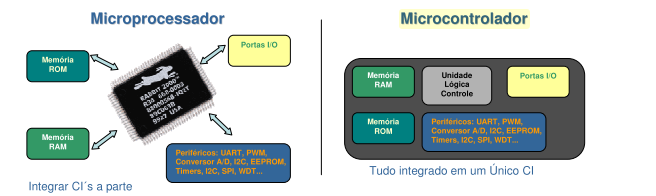
\includegraphics[scale=0.7]{figuras/processa-controla.png}
	\caption{Arquitetura básica de microprocessadores e microcontroladores.}
	\legend{Fonte: \citeauthor{chase2007sistemas} (\citeyear{chase2007sistemas})}
	\label{fig:microprocessador-microcontrolador}
\end{figure}

\newpage

%O microcontrolador a ser utilizado no projeto é o ESP8266 (Figura \ref{fig:esp}), que é um circuito integrado, com interfaces de I/O digitais e analógicas. Possui interface Wi-Fi, com um microprocessador de 32 bits, capaz de executar tarefas a 160 MHz.
%
%Os circuitos baseados no microcontrolador ESP8266 representam um grande avanço na relação de preço-recursos e pode ser um componente muito interessante para soluções IoT \cite {de2017internet}.
%
%\begin{figure}[htbp]
%		\centering
%		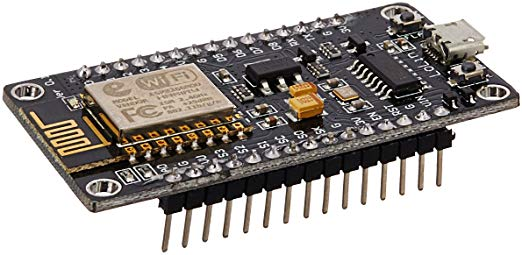
\includegraphics[scale=0.5]{figuras/esp8266_.jpg}
%		\caption{ESP8266.}
%		\legend{Fonte: \citeauthor{Kodali2017} (\citeyear{Kodali2017})}
%		\label{fig:esp}
%\end{figure}


\subsection{Raspberry Pi}

O Raspberry Pi (Figura \ref{fig:rpi}) é um minicomputador criado pela Raspberry Pi Foundation. Seu objetivo é estimular o ensino da ciência da computação nas escolas e universidades. Apesar do Raspberry Pi possuir o hardware em uma única placa eletrônica de tamanho reduzido, seu potencial de processamento é significativo \cite{crotti2013raspberrypi}. O Raspberry Pi pode ser usado em diversos projetos tecnológicos, como experimentos remotos nos quais sua função é ser um micro servidor web \cite{crotti2013raspberrypi}.

\begin{figure}[htbp]
		\centering
		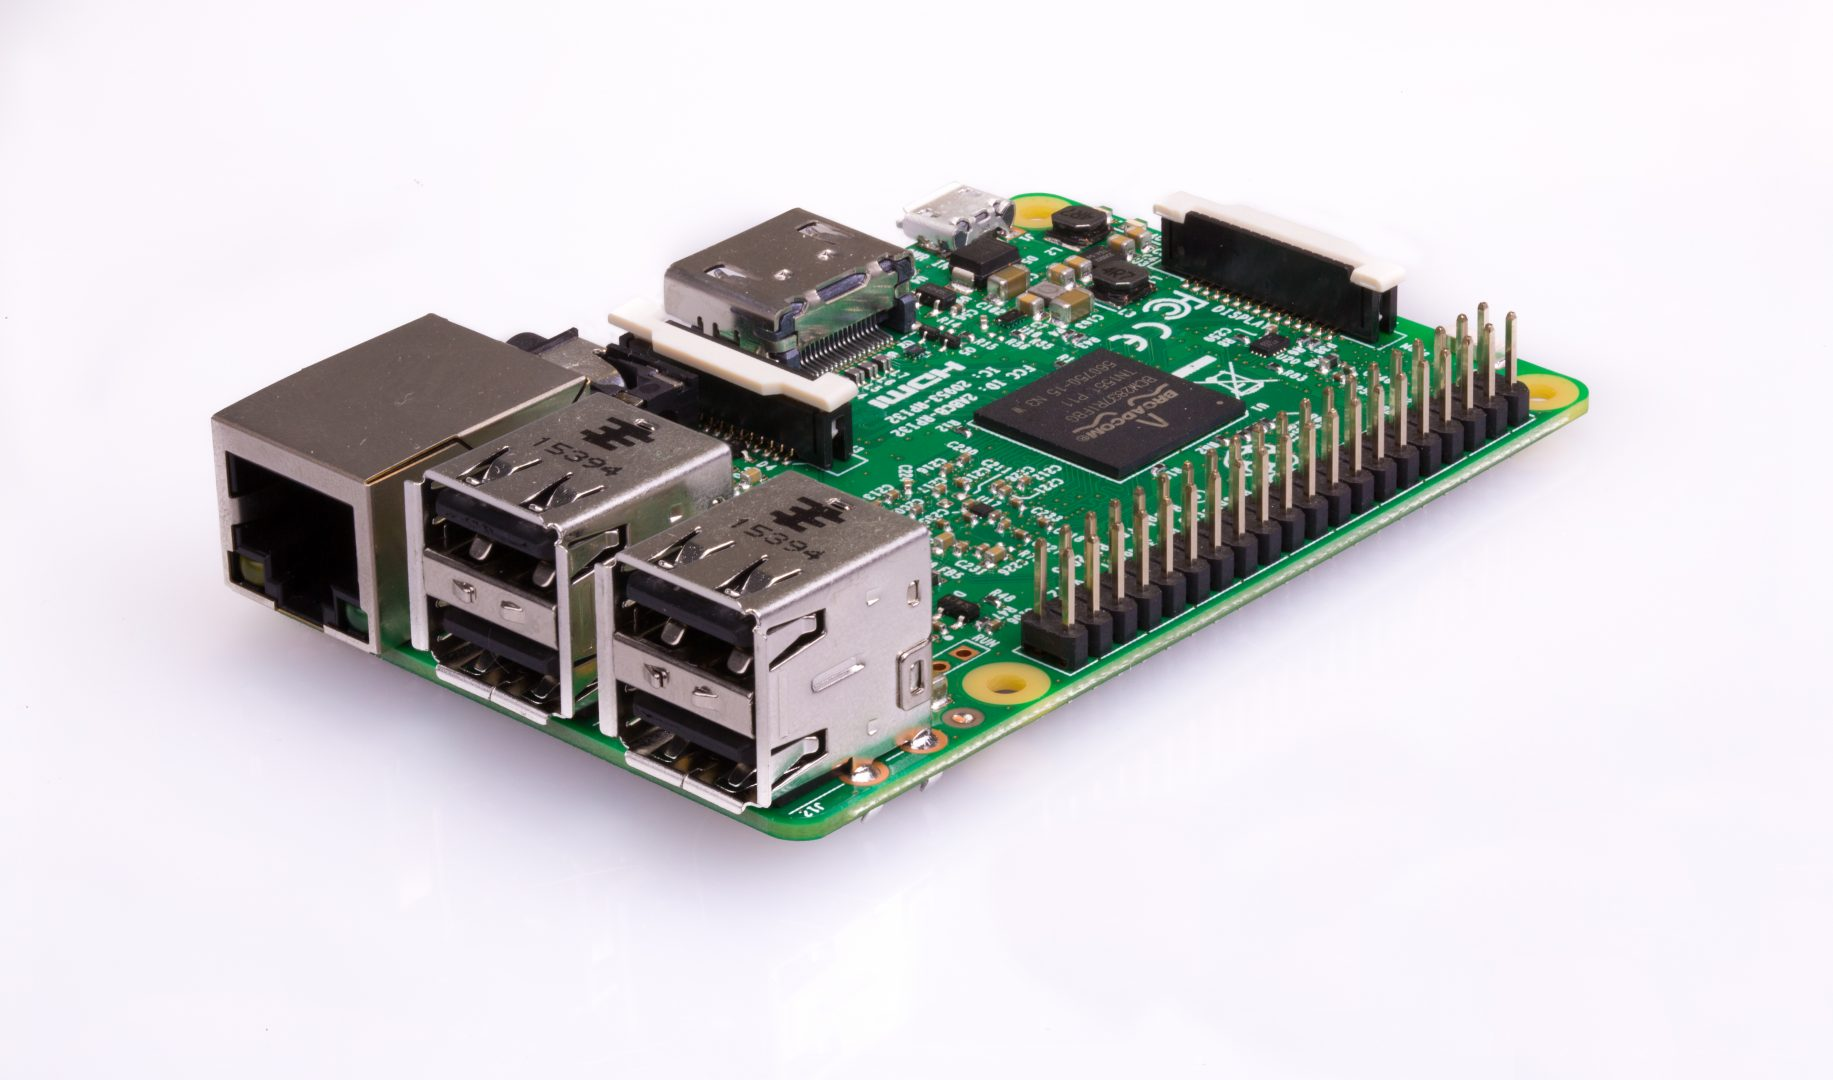
\includegraphics[scale=0.2]{figuras/raspberrypi.jpg}
		\caption{Raspberry Pi.}
		\label{fig:rpi}
\end{figure}

\section{Sensores e atuadores}

Nesta seção serão apresentados os sensores e atuadores a terem seus sinais utilizados no projeto. 

\subsection{Sensor de fluxo YF-S201} \label{sec:sensor}

O sensor YF-S201 (Figura \ref{fig:sensor}) é um sensor do tipo turbina que mede a quantidade de líquido que passa pela tubulação, girando aletas que
geram pulsos de onda quadrada através de um sensor de efeito Hall \cite{roque2018sistema}. O
sensor usa esse efeito para enviar um sinal PWM (\textit{Pulse Width Modulation}) e, através da contagem deste sinal é possível mensurar a quantidade de água que passa pela turbina no interior do sensor. \cite{ms2017automaccao}

\begin{figure}[htbp]
		\centering
		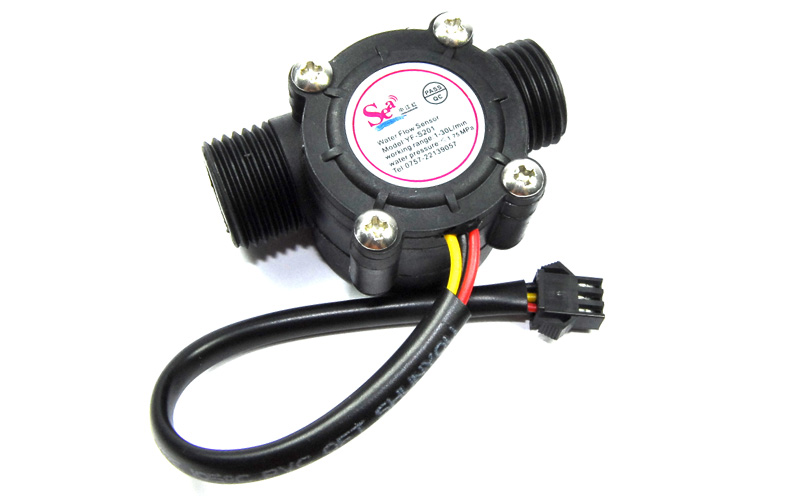
\includegraphics[scale=0.3]{figuras/yf-s201.jpg}
		\caption{Sensor de fluxo de água YF-S201.}
		\label{fig:sensor}
\end{figure}

\newpage

\subsection{Teclado matricial de membrana} \label{sec:teclado}

Teclados permitem que usuários insiram informações em diversos tipos de sistemas, como computadores, calculadoras, controles remotos entre outros \cite{teclado-matricial-1}. O Teclado Matricial de Membrana 4X4 (Figura \ref{fig:teclado}) foi desenvolvido com a finalidade de facilitar a entrada de dados em projetos com plataformas microcontrolada \cite{teclado-matricial}. Este teclado possui 16 teclas, sendo 10 teclas são numéricas, 4 literais e 2 caracteres especiais.

\begin{figure}[htbp]
	\centering
	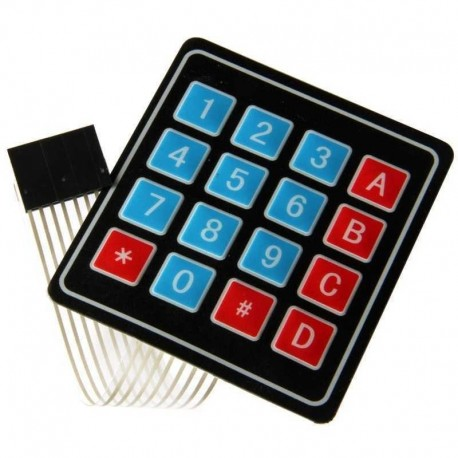
\includegraphics[scale=0.2]{figuras/teclado-matricial.jpg}
	\caption{Teclado Matricial de Membrana.}
	\legend{Fonte: \citeauthor{teclado-matricial-1} (\citeyear{teclado-matricial-1})}
	\label{fig:teclado}
\end{figure}

As teclas estão dispostas em 4 linhas por 4 colunas e o teclado possui um conector de 8 pinos para ligação. Quando um botão do teclado é pressionado, ele conecta a linha com a coluna na qual está ligado, gerando um sinal nos pinos referente àquela linha/coluna. Este sinal permite a identificação da tecla apertada pelo sistema. O circuito do teclado está exemplificado na Figura \ref{fig:teclado-conexoes}.

\begin{figure}[htbp]
	\centering
	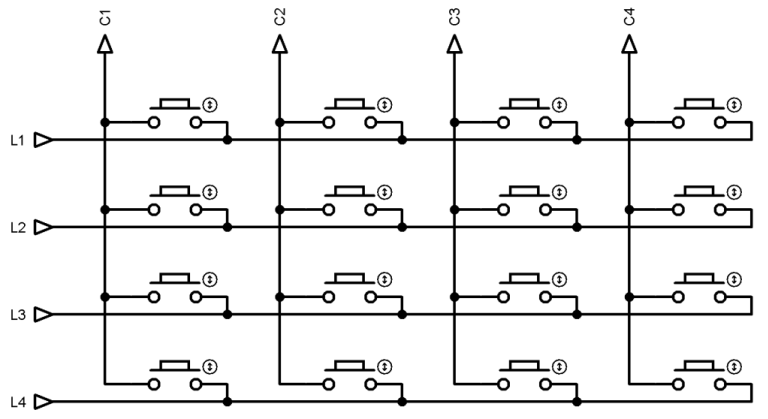
\includegraphics[scale=0.4]{figuras/matrix-1024x558.png}
	\caption{Circuito do teclado.}
	\legend{Fonte: \citeauthor{teclado-matricial} (\citeyear{teclado-matricial})}
	\label{fig:teclado-conexoes}
\end{figure}

A Tabela \ref{table:pinosteclado} possui as informações da distribuição dos pinos em tabelas e colunas, exemplificada na Figura \ref{fig:teclado-pins}.

\begin{table}[h!]
	\begin{center}
		\begin{tabular}{ |c|c| }
			\hline
			\rowcolor{lightgray} Pino & Localização \\
			 \hline 
				1 & Linha 1 \\
			 \hline 
				2 & Linha 2 \\
			 \hline 
				3 & Linha 3 \\
			 \hline 
				4 & Linha 4 \\
			 \hline 
				5 & Coluna 1 \\
			 \hline 
				6 & Coluna 2 \\
			 \hline 
				7 & Coluna 3 \\
			 \hline 
				8 & Coluna 4 \\
			\hline
		\end{tabular}
	\caption{Tabela de disposição dos pinos do teclado numérico.}
	\label{table:pinosteclado}
	\end{center}
\end{table}

\begin{figure}[htbp]
	\centering
	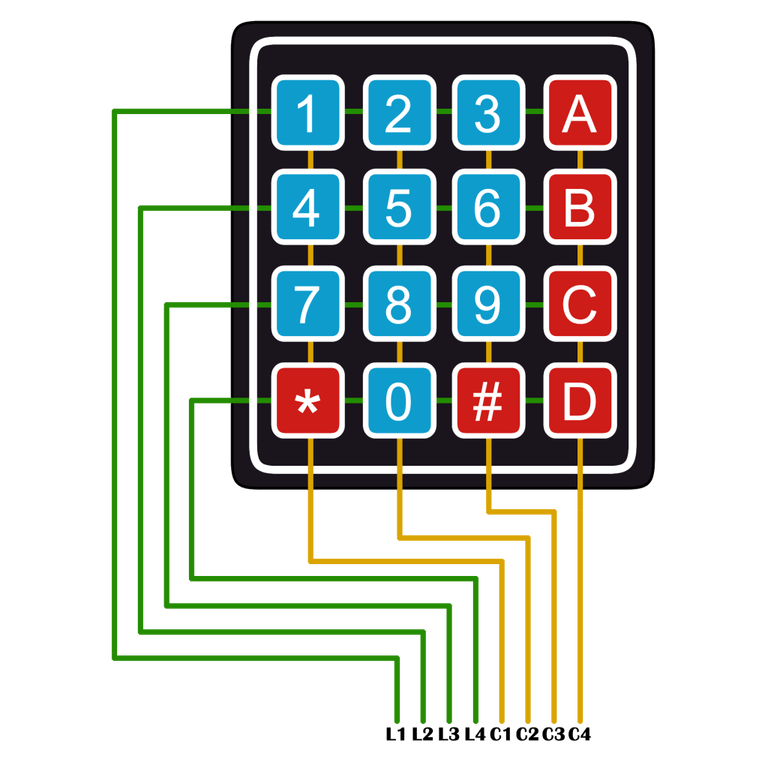
\includegraphics[scale=0.3]{figuras/keypad-1024x1024-pins.png}
	\caption{Pinagem do teclado.}
	\legend{Fonte: \citeauthor{teclado-matricial} (\citeyear{teclado-matricial})}
	\label{fig:teclado-pins}
\end{figure}

\newpage

\subsection{Válvula solenoide} \label{sec:valvula}

Solenóides são dispositivos eletromecânicos baseados no deslocamento causado pela ação de um campo magnético gerado por uma bobina e são muito utilizados na construção de outros dispositivos, como é o caso das válvulas para controle de fluidos. Em particular, as válvulas para baixas vazões (da ordem de mililitros por minuto) e baixas pressões têm sido amplamente aplicadas em equipamentos e montagens para uso em laboratórios clínicos e químicos  \cite{da2002modulo}. Elas são de pequenas dimensões e requerem baixa tensão e corrente de acionamento.

A válvula solenoide pode ser vista na Figura \ref{fig:valvula-solenoide}.

\begin{figure}[htbp]
	\centering
	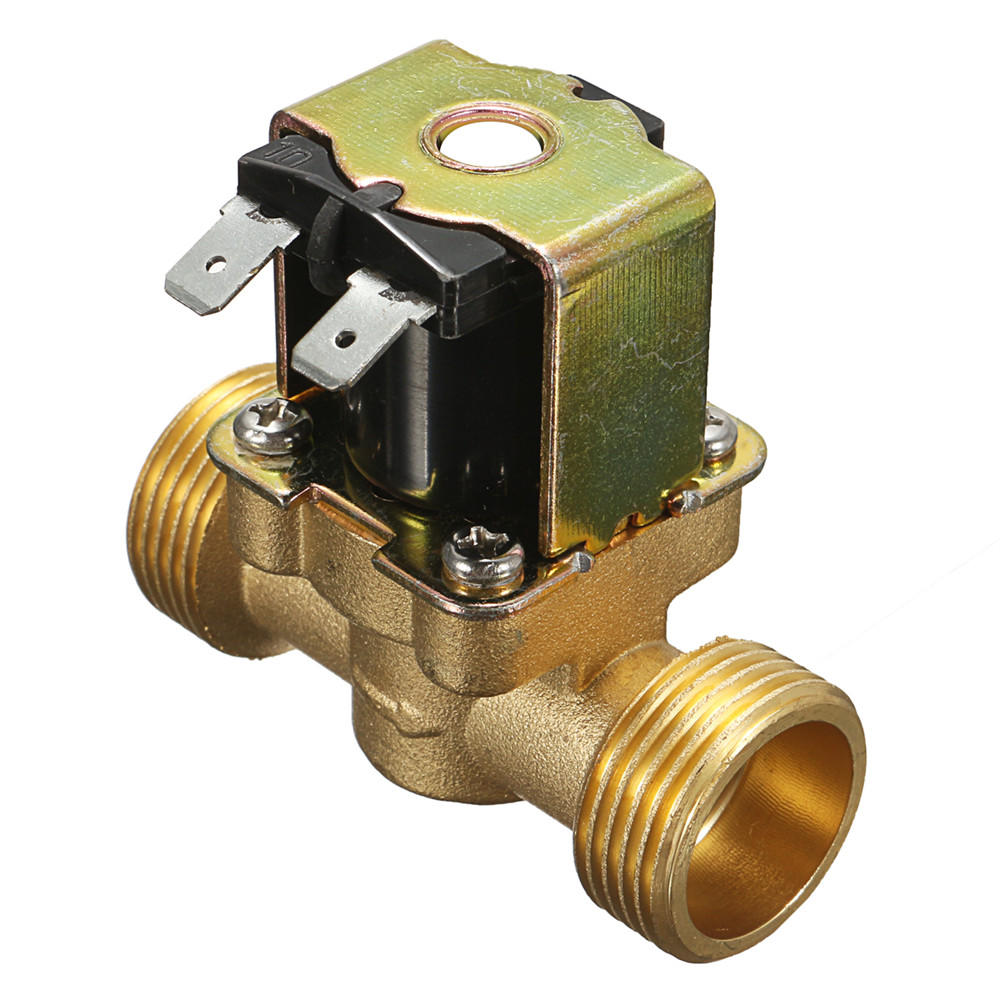
\includegraphics[width=0.3\linewidth]{figuras/valvula-solenoide.jpg}
	\caption{Válvula Solenoide.}
	\label{fig:valvula-solenoide}
\end{figure}

Segundo \citeauthor{da2002modulo} (\citeyear{da2002modulo}), a estratégia para fechamento e abertura dos canais fluídicos depende do fabricante, mas o princípio de acionamento elétrico é comumente o mesmo. Uma tensão é aplicada sobre um solenoide, criando um campo magnético que desloca um núcleo ferromagnético móvel, causando a alteração do estado da válvula. O núcleo
ferromagnético comprime uma mola que é a responsável por retornar o núcleo a sua posição original quando a corrente elétrica é interrompida.

\section{Softwares}

Os softwares que foram utilizados para a implementação do sistema estão presentes nesta seção.

\subsection{HomeAssistant}

O HomeAssistant é um plataforma de automação escrita em Python. Inclui componentes contribuídos por usuários que permite a interface com Web Services e dispositivos como sensores, microcontroladores e assistentes virtuais \cite{Lundrigan2017}. Em seu núcleo, o HomeAssistant é um protocolo de troca de mensagens que facilita a comunicação entre dispositivos e componentes funcionais na rede. Provendo simples abstrações de componentes de automação residencial como sensores, câmeras, \textit{players} de música, etc.

A Figura \ref{fig:homeassistant-dash} apresenta um exemplo de tela inicial do HomeAssistant. Com vários sensores configurados na parte superior, na parte esquerda, encontra-se o menu do HomeAssistant, e na parte central inferior pode-se observar informações sobre o clima e \textit{switches} para acionamento de interruptores e iluminação.

\begin{figure}[htbp]
	\centering
	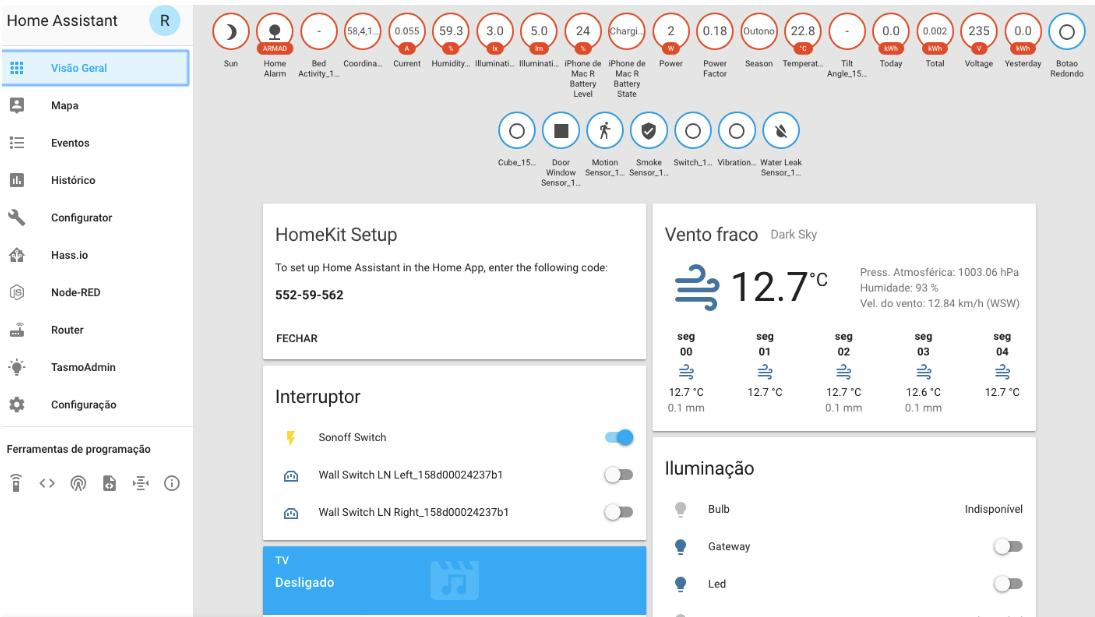
\includegraphics[width=1\linewidth]{figuras/homeassistant-dash.png}
	\caption{Dashboard genérico do HomeAssistant}
	\legend{Fonte: Adaptado de \citeauthor{AlmeidaCosta} (\citeyear{AlmeidaCosta})}
	\label{fig:homeassistant-dash}
\end{figure}

O HomeAssistant tem suporte para diversos tipos de protocolos \textit{wireless}, como BLE, ZigBee, Z-Wave e Wi-Fi. Conta também com um RESTful API e suporta HTTP, MQTT, TCP \textit{sockets} e componentes customizados. Estes componentes customizados permitem aos usuários adicionar funções próprias no HomeAssistant sem a necessidade de mudar o seu código fonte. Isto torna a integração de novos dispositivos e sensores muito mais fácil com o HomeAssistant \cite{Gomes2018}.


%O HomeAssistant conta com uma grande comunidade de desenvolvedores com mais de 1.450 contribuidores e 23.700 estrelas no GitHub\footnote{\url{https://github.com/home-assistant/home-assistant}}, o que significa uma abundância em sua documentação sobre os seus componentes, fóruns e chats para conseguir ajuda de outros usuários, e diversos posts em blogs e vídeos sobre como começar a utilizar o programa.

Tendo em vista a gama de protocolos sem fio disponíveis no HomeAssistant, escolhemos o padrão Wi-Fi pois segundo \citeauthor{Lundrigan2017} (\citeyear{Lundrigan2017}):

\begin{itemize}
	\item O custo dos equipamentos com padrão Wi-Fi é reduzido.
	\item Wi-Fi é o mais difuso dos protocolos wireless.
	\item Sensores Wi-Fi tem integração facilitada com demais equipamentos residenciais.
\end{itemize}

O HomeAssistant pode ser instalado em qualquer sistema operacional devido ao fato de ser muito pequeno e leve. O que o faz ser compatível para o uso no Rasberry Pi como um hub de automação pequeno e barato. É importante lembrar que o HomeAssistant age apenas como uma central de controle que pode informar outros serviços, como o Philips Hue ou o Nest, que são produtos para automação residencial, para realizar alguma função \cite{AlmeidaCosta}. O Home Assistant é gratuito e de fácil configuração.

\subsection{Banco de dados de séries temporais}

Um Banco de Dados de Séries Temporais, do inglês \textit{Temporal Series Database} (TSDB), é um tipo de banco otimizado para dados coletados no tempo. É implementado especificamente para lidar com métricas, eventos ou medidas que variam no tempo. Um TSDB permite o usuário criar, enumerar, alterar, destruir e organizar várias séries temporais de métodos mais eficientes. Atualmente, a maioria das empresas estão gerando um grande volume de dados sobre métricas e eventos que são mapeados no tempo, aumentando a relevância de tal arquitetura \cite{Noor2017}.

Ainda segundo \citeauthor{Noor2017} (\citeyear{Noor2017}), aplicações comuns para os TSDBs são IoT, DevOps e Analise de Dados. Alguns casos de uso incluem monitoramento de sistemas de \textit{software} como máquinas virtuais, monitoramento de sistemas físicos como dispositivos, ambiente, sistemas de automação residencial, dentre outros.

\subsubsection{InfluxDB}

O InfluxDB é o Banco de Dados de Séries Temporais usado neste projeto, sendo o mais apto a guardar os dados de fluxo no tempo. \cite{Lundrigan2017}

É um projeto \textit{open-source} com o opcional de armazenamento pago em nuvem desenvolvido pela empresa InfluxData. É escrito na linguagem de programação Go e baseado em uma linguagem de consulta parecida com o SQL \cite{Noor2017}.

\subsubsection{Grafana}

Grafana é um projeto \textit{open-source} para análise de dados de séries temporais  \cite{Noor2017} que realiza consultas destas séries temporais a partir do InfluxDB exibindo os dados de maneira gráfica \cite{chang2017kubernetes}.

\subsection{Banco de dados relacional}

Um Banco de Dados Relacional é capaz de salvar e referenciar dados para uma consulta posterior. Possui uma coleção de tabelas, todas com identificadores únicos, que compõem a base de
dados. Conceitos como integridade referencial de dados – que garante sincronia de dados entre tabelas – e chaves primárias estão presentes, garantindo que um conjunto de informações possa ser representado de maneira consistente, independente da forma de acesso  \cite{bancosrelacionais}.

\subsubsection{PostgreSQL}

O PostgreSQL é uma implementação de um banco de dados relacional, de código aberto e de custo gratuito \cite{stones2006beginning}. O 
PostgreSQL pode ser usado com diversas linguagens de programação, como por exemplo: Python, Javascript, Java e C++.

O PostgreSQL ganhou diversos prêmios, incluindo o \textit{Linux Journal Editor's Choice Award for Best Database} três vezes e o \textit{2004 Linux New Media Award for Best Database System}.

\subsection{Node.JS}

O Node.JS, também chamado de Node, é um ambiente de servidor que utiliza a linguagem de programação JavaScript. É baseado no \textit{runtime} do Google, chamado de motor V8. O V8 e o Node são implementados em C e C++, focados no desempenho e baixo consumo de memória. Embora o V8 suporte principalmente o uso de JavaScript no navegador, o Node foca no suporte de processos de servidores \cite{Tilkov2010}.

O Node.JS utiliza um paradigma baseado em eventos e não-bloqueador de I/O, o que o torna leve e eficiente. É perfeito para aplicações de tempo real que lidam com dados intensos em dispositivos de baixo poder de processamento \cite{Sapes2016}.

O Node é um dos ambientes e \textit{frameworks} mais famosos que suportam o desenvolvimento de servidores utilizando o JavaScript. A comunidade criou um grande ecossistema de bibliotecas e vasta documentação de suporte ao Node \cite{Tilkov2010}.

\subsection{Arquitetura de microsserviços}

Seguindo a definição de \citeauthor{ms1} (\citeyear{ms1}), a arquitetura de microsserviços trata do desenvolvimento de uma aplicação que baseia na existência de diversos pequenos serviços independentes. Cada um dos serviços deve rodar em seu próprio processo independente. Estes serviços podem comunicar entre si utilizando mecanismos leves de comunicação (geralmente em torno no HTTP). Os serviços devem ser absolutamente independentes.

Um exemplo da arquitetura de microsserviços está na Figura \ref{fig:arquitetura-microsservicos}.

\begin{figure}[htbp]
	\centering
	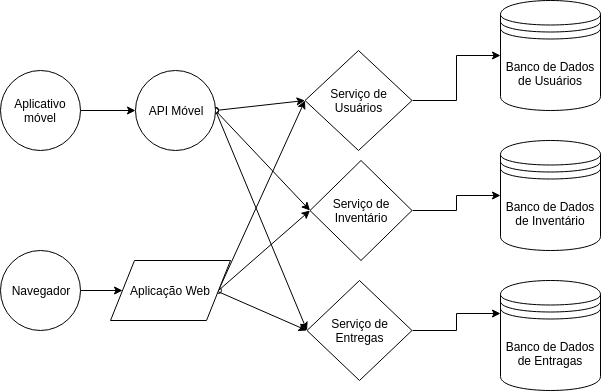
\includegraphics[width=1\linewidth]{figuras/Microservice_Architecture.png}
	\caption{Exemplo arquitetura de microsserviços.}
	\label{fig:arquitetura-microsservicos}
\end{figure}

Microsserviços são os resultados da decomposição funcional de uma aplicação. São caracterizados pela definição de sua interface e função no sistema. Como cada serviço deve ser independente, uma alteração na sua implementação não deve afetar o funcionamento dos demais. \cite{Pahl}

\subsection{Protocolo de comunicação MQTT}

MQTT significa \textit{Message Queuing Telemetry Transport}, traduzido para o português como Transporte de Telemetria de Enfileiramento de Mensagens. É um protocolo de transporte leve que otimiza o uso da a largura de banda de rede\footnote{\url{http://public.dhe. ibm.com/software/dw/webservices/ws-mqtt/mqtt-v3r1.html}}. O MQTT trabalha sobre o protocolo TCP e garante a entrega de mensagens de um nó para um servidor. Sendo um protocolo orientado por troca de mensagens, MQTT é ideal para aplicações IoT, que comumente tem recursos e capacidades limitados.

É um protocolo inicialmente desenvolvido pela IBM\footnote{\url{http://www.hivemq.com/blog/mqtt-essentials-part-1-introducing-mqtt}} em 1999, sendo recentemente reconhecido como padrão pela OASIS (Organizarion for the Advancement of Structured Information Standards)\footnote{\url{https://www.oasis-open.org/news/announcements/ mqtt-version-3-1-1-becomes-an-oasis-standard}}.

\citeauthor{Kodali2017} (\citeyear{Kodali2017}) definiu o MQTT como um protocolo baseado em \textit {publisher/subscriber}. Qualquer conexão MQTT envolve dois tipos de agentes, os clientes e um \textit {broker}, ou servidor. Qualquer dispositivo ou programa que é conectado pela rede e troca mensagens através do MQTT é chamado de cliente. Um cliente pode ser tanto um \textit {publisher} e/ou um \textit {subscriber}. Um \textit {publisher} publica mensagens e um \textit {subscriber} requisita o recebimento de mensagens. Um MQTT \textit {server} é um programa que interconecta os clientes. Ele aceita e transmite as mensagens através de múltiplos clientes conectados à ele.

\begin{figure}[htbp]
	\centering
	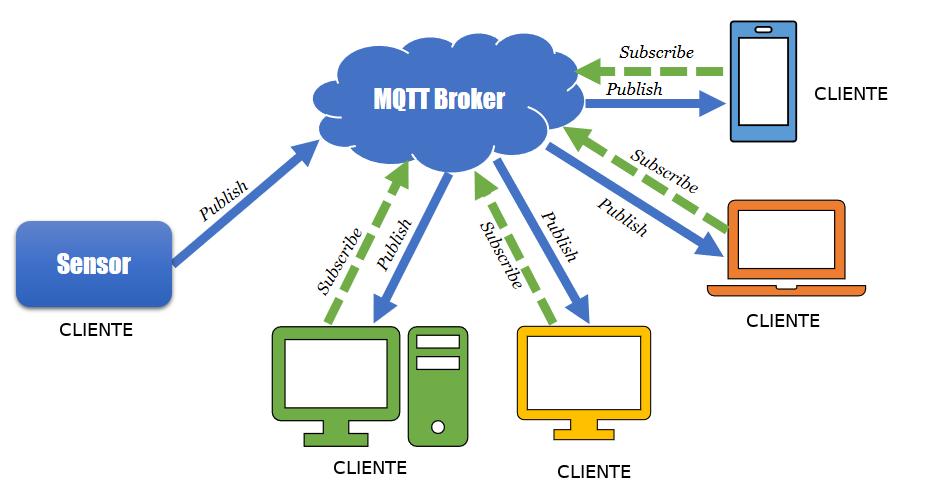
\includegraphics[width=1\linewidth]{figuras/mqtt-architecture.png}
	\caption{Exemplo da arquitetura do MQTT.}
	\legend{Fonte: \citeauthor{embeddedmqtt} (\citeyear{embeddedmqtt})}
	\label{fig:arquitetura-mqtt}
\end{figure}

\newpage

Dispositivos como sensores e celulares podem ser vistos como clientes do ponto de vista da arquitetura MQTT. Quando um cliente tem alguma informação para transmitir, ele publica o dado para o \textit {broker}.

A Figura \ref{fig:arquitetura-mqtt} apresenta um exemplo de arquitetura MQTT comum. O \textit {broker} MQTT, ou servidor MQTT é responsável por coletar e organizar os dados. As mensagens publicadas por clientes MQTT são transmitidas para outros clientes MQTT que se inscreverem ao tópico. O MQTT é desenhado para simplificar a implementação no cliente por concentrar todas as complexidades no \textit {broker}. Os \textit {publishers} e \textit {subscribers} são isolados, o que significa que eles não precisam conhecer a existência do outro.

\subsubsection{MQTT Mosquitto}

O Mosquitto é um \textit{broker} MQTT de código aberto \cite{Kodali2017} que entrega uma implementação de servidor e cliente MQTT. Utiliza o modelo \textit{publisher/subscriber}, tem uma baixa utilização de rede e pode ser implementado em dispositivos de baixo custo como microcontroladores. \cite{Light}

Segundo \citeauthor{Light} (\citeyear{Light}), Mosquitto é recomendado para o uso sempre em que se necessita de mensagens leves, particularmente em dispositivos com recursos limitados.

O Projeto Mosquitto é um membro da Eclipse Foundation. Existem três partes no projeto:

\begin{itemize}
	\item O servidor principal Mosquitto.
	\item Os clientes mosquitto \textit{pub} e mosquitto \textit{sub}, que contém ferramentas para se comunicar com o servidor MQTT.
	\item Uma biblioteca cliente MQTT, escrita em C.
\end{itemize}

%\subsection{Docker}
%
%Docker é um projeto \textit{open source} que foi inicialmente lançado em 2013, atraiu grande atenção na industria de TI. É uma plataforma de conteinerização que possibilita usuários a construir sua aplicação dentro de um conteiner e transferir conteiners através de máquinas com diferentes sistemas operacionais de um jeito simples. \cite{chang2017kubernetes}
%
%Existem três componentes principais do Docker:
%
%\begin{itemize}
%	\item \textit{Docker images}: são \textit{templates} de leitura que servem como base para a criação de conteiners.;
%	\item \textit{Docker registries}: é o local onde estão uma grande coleção de \textit{Docker images}.;
%	\item \textit{Docker containers}: são as instâncias virtuais em que as aplicações estão rodando. Cada conteiner contem uma aplicação rodando e todas os seus arquivos de dependências, como o código, bibliotecas e utilitários do sistema.
%\end{itemize}
%
%A construção de imagens pode ser feita de duas maneiras. É possível criar um conteiner através de uma imagem já existente (\textit{docker run}), realizar modificações e instalações dentro do conteiner, parar o container e depois salvar o estado atual do conteiner como uma nova imagem (\textit{docker commit}). Este processo é parecido com uma instalação clássica de uma máquina virtual, mas deve ser feito para cada imagem caso haja alguma atualização, já que as imagens são padronizadas. Para automatizar o processo, \textit{Dockerfiles} nos permite especificar uma imagem de base e uma sequência de comandos que serão executados quando a imagem é construída, juntamente com outras opções de especificações, como portas a serem expostas. A imagem é depois construída com o comando \textit{docker build}.\cite{DiPietro}

% ----------------------------------------------------------
% PARTE
% ----------------------------------------------------------
%\part{Metodologia}
% ----------------------------------------------------------
% ---
% Capitulo de metodologia
% ---
\chapter{Metodologia}

Este Capítulo apresenta a estrutura geral do sistema, a configuração inicial do Raspberry Pi, a construção dos microsserviços, assim como as etapas de realização do projeto. A
primeira etapa consiste no desenvolvimento do microsserviço de cadastro e controle de usuários. Em seguida, foi desenvolvido o sistema que recebe os dados via MQTT, guardando-os no InfluxDB. Com os dados sendo recebidos e devidamente guardados, foram configurados o HomeAssistant e Grafana.

A validação do projeto será feita através de um sistema criado para emular os dados vindos dos sensores, atuadores e teclado. %Este sistema é capaz de criar dados que simulam os sinais recebidos pelo sensor YF-S201, pelo teclado numérico e atuador.

\section{Funcionamento do sistema} \label{sec:funcionamento}

Nesta seção estão descritos os parâmetros utilizados pelo sistema, os dados que são gerados, assim como as respostas esperadas. A arquitetura geral do sistema pode ser visualizada na Figura \ref{fig:arqgeral}, mostrando os sistemas desenvolvidos, os tópicos do servidor MQTT e os sistemas que implementam os bancos de dados.

\begin{figure}[htbp]
	\centering
	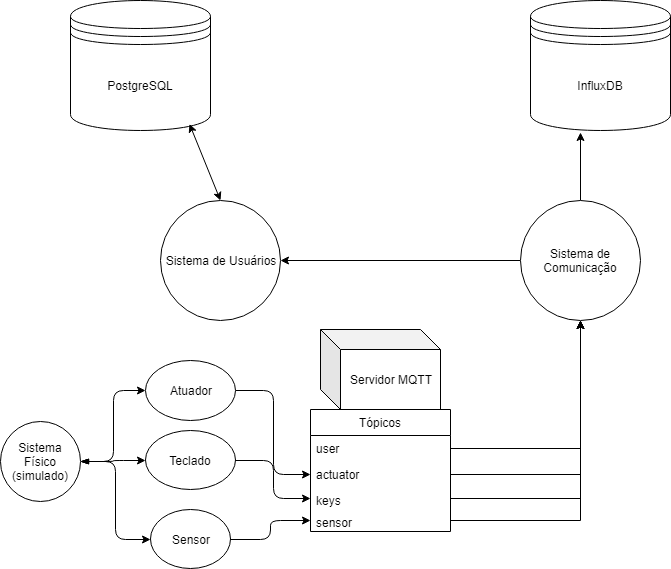
\includegraphics[width=0.7\linewidth]{figuras/arquiteturaprojeto.png}
	\caption{Arquitetura geral do projeto.}
	\label{fig:arqgeral}
\end{figure}

\subsection{Parâmetros de operação}

Os parâmetros de operação são utilizados pelo sistema para garantir o funcionamento esperado. Estes parâmetros são:

\begin{itemize}
	\item Tempo de banho permitido: é o tempo máximo de banho permitido para cada usuário;
	\item Estado do chuveiro: ligado ou desligado;
	\item Estado do usuário: autorizado ou não autorizado;
\end{itemize}

Ao se criar um usuário é necessário informar três dados: nome do usuário, senha e tempo de banho permitido. A senha é utilizada para autorizar o usuário a tomar o banho, para iniciar o banho, o usuário deve digitar sua senha no teclado numérico. O tempo de banho permitido é o tempo máximo em que o chuveiro pode ficar ligado; ao exceder este limite, o atuador irá interromper o fluxo de água.

O estado do chuveiro poderá ser observado no HomeAssistant, que dirá se o usuário está com o chuveiro ligado ou desligado. O HomeAssistant proverá  informações personalizadas de acordo com o usuário.

\subsection{Dados gerados}

O usuário, ao digitar a sua senha correta no teclado numérico, liberará o atuador e o fluxo de água começará a passar pelo sensor de fluxo. Este sensor irá gerar dados que dizem informações a respeito do fluxo volumétrico de água passado por ele.

Os dados do sensor são gravados no InfluxDB e poderão ser vistos no Grafana em forma de gráfico, sendo possível distinguir os usuários. O sistema, ao perceber uma parada no fluxo, ou se o tempo de banho ultrapassar o limite de banho do usuário, fecha o atuador e contabiliza o tempo total do banho tomado, salvando-o no Banco de Dados PostgreSQL.

\subsection{Ligar/desligar atuador}

Para ligar o atuador, o sistema necessita identificar o usuário e autenticá-lo. Esta identificação e autenticação é realizada via teclado numérico. O usuário é identificado pelo seu id, que é fornecido no momento do seu cadastro. Para realizar a identificação, o usuário deve pressionar a tecla \textit{*} seguido pelo seu id e \textit{\#}. Ao realizar a consulta, o sistema retorna o nome do usuário e requisita a senha.

Após digitar a senha, a tecla \textit{\#} deve ser pressionada e o sistema irá comparar a senha digitada com a cadastrada no banco de dados. Caso as senhas forem iguais, o atuador é ligado; caso forem diferentes, o sistema retorna que o usuário não está autenticado e não liga o atuador. 

A Figura \ref{fig:mockservice} mostra este fluxo de digitação, assim como a identificação do usuário pelo id.

\section{Configuração do Raspberry Pi} \label{sec:confrasp}

Para a configuração inicial do Raspberry Pi é preciso fazer o download de um sistema operacional compatível com o microcontrolador. Para o sistema deste projeto, utilizamos o Hassbian\footnote{\url{https://www.home-assistant.io/docs/installation/hassbian/installation/}}, que foi instalado no cartão SD a ser inserido no Raspberry Pi.


Os sistemas deste projeto foram desenvolvidos diretamente no Raspberry Pi e, para possibilitar este desenvolvimento, é necessário primeiramente configurar o ambiente do Raspberry Pi.

O Raspberry Pi foi configurado para ser \textit{headless}\footnote{\url{https://www.raspberrypi.org/documentation/configuration/wireless/headless.md}}, o que faz com que ele não necessite de teclado, mouse ou monitor para poder ser acessado. Para conseguir acessar o Raspberry Pi nesta configuração é necessária a utilização do SSH, ou \textit{Secure Shell}, que é um protocolo de rede criptográfico para operação de serviços de rede de forma segura\footnote{\url{https://www.ssh.com/ssh/}}. O SSH permite o login remoto no sistema operacional do Raspberry, possibilitando o completo controle do sistema operacional de forma remota.

A configuração de rede do Raspberry Pi foi realizada para conter um IP estático (\textit{192.168.2.60}), que facilita o acesso SSH ao sistema.

O Código \ref{cod:headless} mostra um exemplo do arquivo \textit{wpa\_supplicant.conf}, que faz parte da configuração \textit{headless}, servindo para conectar à rede automaticamente ao iniciar os Raspberry Pi. Já no Código \ref{cod:static}, podemos observar a configuração do ip estático.

\begin{lstlisting}[caption=Exemplo de configuração \textit{headless}, label=cod:headless]
update_config=1
ctrl_interface=\var\run\wpa_supplicant

network={
    ssid="<Nome da sua rede Wi-Fi>"
    psk="<Senha da sua rede Wi-Fi>"
}
\end{lstlisting}

\newpage

\begin{lstlisting}[caption=Exemplo de configuração do IP estático, label=cod:static]
update_config=1
interface <Sua interface de rede>
static ip_adress=192.168.2.60
static routers=192.168.2.1
static domain_name_servers=192.168.2.1
\end{lstlisting}

%\begin{figure}[htbp]
%	\centering
%	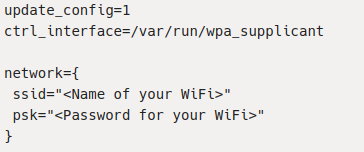
\includegraphics[width=0.6\linewidth]{figuras/headless.png}
%	\caption{Exemplo de configuração \textit{headless}}
%	\label{fig:headless}
%\end{figure}

%\begin{figure}[htbp]
%	\centering
%	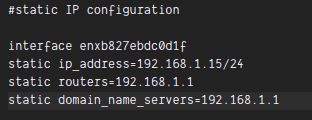
\includegraphics[width=0.6\linewidth]{figuras/rpiip.png}
%	\caption{Exemplo de configuração do IP estático}
%	\label{fig:rpiip}
%\end{figure}

\section{Criação das tabelas no PostgreSQL}

Todos os dados de um banco de dados relacional são armazenados em tabelas. Uma tabela é uma simples estrutura de linhas e colunas. Em um banco de dados podem existir uma ou centenas de tabelas, sendo que o limite pode ser imposto tanto pela ferramenta de \textit{software} utilizada, quanto pelos recursos de hardware disponíveis no equipamento.

As tabelas associam-se entre si por meio de regras de relacionamentos, que consistem em associar um ou vários atributos de uma tabela com um ou vários atributos de outra tabela.

A Figura \ref{fig:erpostgre} mostra o diagrama Entidade Relacionamento do banco de dados \textit{users} criado para a aplicação. Um diagrama Entidade Relacionamento é capaz de descrever um modelo de tabelas (entidades) que são ligadas umas as outras por relacionamentos que expressam as dependências e exigências entre si. No caso do sistema planejado, existem três entidades: Usuário, Configuração e Banho. O usuário se relaciona com as outras duas entidades: ele possui uma configuração e pode tomar um banho.

\begin{figure}[htbp]
	\centering
	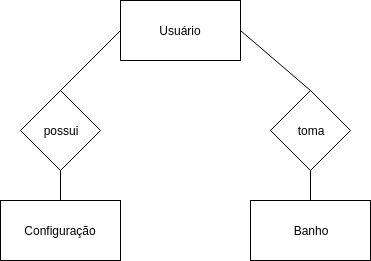
\includegraphics[width=0.6\linewidth]{figuras/ERPostgre.png}
	\caption{Modelo Entidade Relacionamento do PostgreSQL}
	\label{fig:erpostgre}
\end{figure}

\newpage

Para o sistema desenvolvido, foi criado um banco de dados com o nome \textit{users} com três tabelas: \textit{user\_baths}, \textit{user\_settings} e \textit{users}.

A tabela \textit{users} contém 5 colunas que guardam informações dos usuários cadastrados, que são mostradas na Tabela \ref{tab:users}.

%\begin{itemize}
%	\item id: gera um id que se auto incrementa e é único para cada usuário;
%	\item \textit{name}: referente ao nome do usuário;
%	\item \textit{password}: informação da senha do usuário, que é criptografada;
%	\item \textit{created\_at}: data e hora da criação do usuário;
%	\item \textit{updated\_at}: data e hora da ultima atualização do usuário;
%\end{itemize}

\begin{table}[]
	\centering
	\begin{tabular}{|l|l|}
		\hline
		\rowcolor[HTML]{ECF4FF} 
		\multicolumn{1}{|c|}{\cellcolor[HTML]{ECF4FF}Coluna} & \multicolumn{1}{c|}{\cellcolor[HTML]{ECF4FF}Função} \\ \hline
		id                                                   & identificador único que se auto incrementa          \\ \hline
		\textit{name}                                        & nome do usuário cadastrado                          \\ \hline
		\textit{password}                                    & senha criptografada do usuário cadastrado           \\ \hline
		\textit{created\_at}                                 & data e hora da criação do usuário                   \\ \hline
		\textit{updated\_at}                                 & data e hora da última atualização no usuário        \\ \hline
	\end{tabular}
	\caption{Colunas da tabela \textit{users}.}
	\label{tab:users}
\end{table}

A Tabela \ref{tab:user-settings} é a implementação da \textit{user\_settings}, que guarda informações de configuração dos usuários, e também contém 5 colunas.

%\begin{itemize}
%	\item id: identificador único;
%	\item \textit{user\_id}: referente ao id do usuário;
%	\item \textit{allowedBathTime}: tempo de banho permitido do usuário;
%	\item \textit{created\_at}: data e hora da criação do usuário;
%	\item \textit{updated\_at}: data e hora da ultima atualização do usuário;
%\end{itemize}

\begin{table}[]
	\centering
	\begin{tabular}{|l|l|}
		\hline
		\rowcolor[HTML]{ECF4FF} 
		\multicolumn{1}{|c|}{\cellcolor[HTML]{ECF4FF}Coluna} & \multicolumn{1}{c|}{\cellcolor[HTML]{ECF4FF}Função} \\ \hline
		id                                                   & identificador único que se auto incrementa          \\ \hline
		\textit{user\_id}                                    & referência ao id do usuário                         \\ \hline
		\textit{allowed\_bath\_time}                         & tempo máximo de banho permitido                     \\ \hline
		\textit{created\_at}                                 & data e hora da criação do usuário                   \\ \hline
		\textit{updated\_at}                                 & data e hora da última atualização no usuário        \\ \hline
	\end{tabular}
	\caption{Colunas da tabela \textit{user\_settings}.}
	\label{tab:user-settings}
\end{table}

A tabela \textit{user\_baths} guarda informações de tempo de todos os banhos tomados, possuindo 5 colunas, mostradas na Tabela \ref{tab:user-baths}.

%\begin{itemize}
%	\item id: identificador único;
%	\item \textit{user\_id}: referente ao id do usuário;
%	\item \textit{time}: tempo total do banho, em milissegundos;
%	\item \textit{created\_at}: data e hora da criação do usuário;
%	\item \textit{updated\_at}: data e hora da ultima atualização do usuário;
%\end{itemize}

\begin{table}[]
	\centering
	\begin{tabular}{|l|l|}
		\hline
		\rowcolor[HTML]{ECF4FF} 
		\multicolumn{1}{|c|}{\cellcolor[HTML]{ECF4FF}Coluna} & \multicolumn{1}{c|}{\cellcolor[HTML]{ECF4FF}Função} \\ \hline
		id                                                   & identificador único que se auto incrementa          \\ \hline
		\textit{user\_id}                                    & referência ao id do usuário                         \\ \hline
		\textit{time}                                        & tempo total do banho, em milissegundos              \\ \hline
		\textit{created\_at}                                 & data e hora da criação do usuário                   \\ \hline
		\textit{updated\_at}                                 & data e hora da última atualização no usuário        \\ \hline
	\end{tabular}
	\caption{Colunas da tabela \textit{user\_baths}.}
	\label{tab:user-baths}
\end{table}

A Figura \ref{fig:modeltables} ilustra o banco de dados criado juntamente com as tabelas contidas nele.

\begin{figure}[htbp]
	\centering
	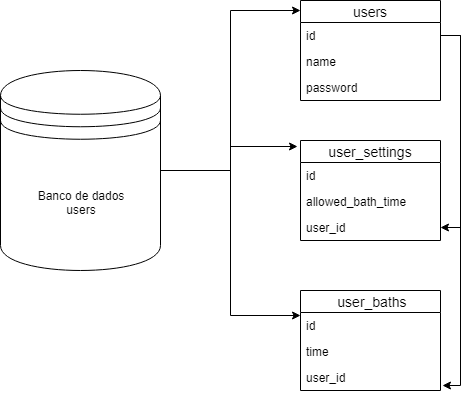
\includegraphics[width=0.6\linewidth]{figuras/postgrediagram.png}
	\caption{Modelo das tabelas criadas no banco de dados}
	\label{fig:modeltables}
\end{figure}

\newpage

\section{Configuração do InfluxDB}

Na configuração do InfluxDB, foi utilizada a biblioteca \textit{influx}\footnote{\url{https://www.npmjs.com/package/influx}}. Esta biblioteca permite a criação do banco de dados diretamente do código fonte do sistema, assim como as tabelas para guardar os dados temporais.

Foi criado o banco de dados \textit{water\_flow\_data}, que guarda os dados temporais dos banhos dos usuários. Neste banco, os dados são guardados com a \textit{tag} referente ao id do usuário cadastrado no banco relacional PostgreSQL. Nos \textit{fields} são guardados os dados que chegam diretamente do sensor, ou seja, o fluxo de água naquele determinado instante.

O InfluxDB salva automaticamente os \textit{timestamps}\footnote{\textit{Timestamps} são marcas temporais, informa a data e a hora que um certo evento ocorreu.} de cada dado incluido nele, o que facilita a manipulação dos dados, pois não é necessário informar a data e a hora toda vez que for incluir algum dado no banco.

No \lstlistingname\ \ref{list:codigoinflux} está um exemplo de configuração e implementação das funções do InfluxDB no sistema.

\newpage

%\begin{figure}[htbp]
%	\centering
%	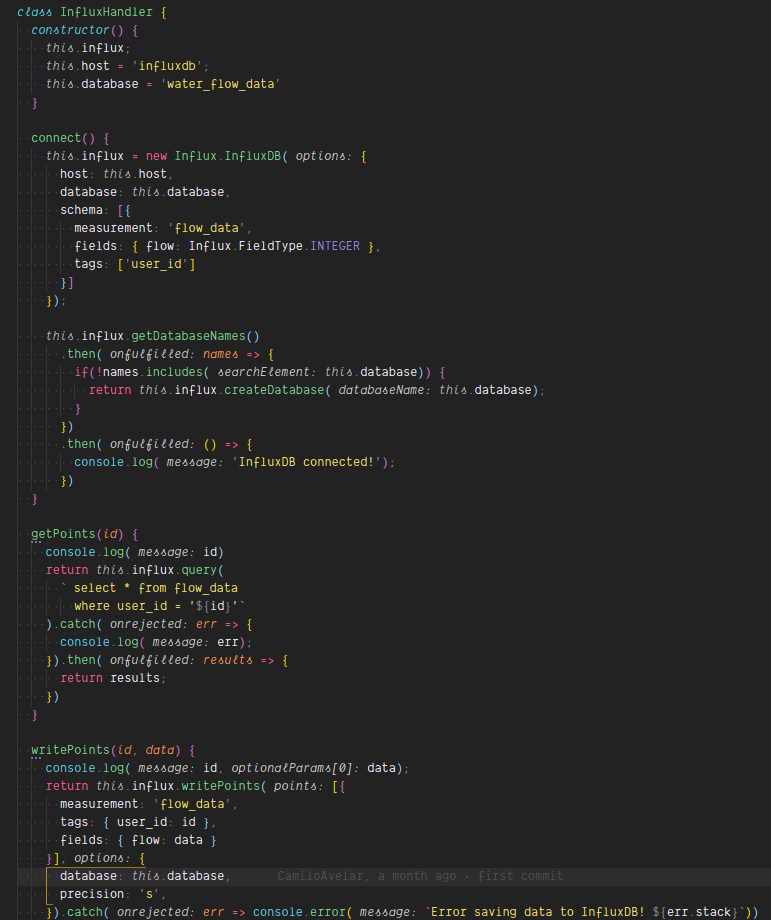
\includegraphics[width=1\linewidth]{figuras/influxconf.png}
%	\caption{Código de configuração do InfluxDB}
%	\label{fig:influxconf}
%\end{figure}

\begin{lstlisting}[label=list:codigoinflux, caption=Exemplo do código de configuração do InfluxDB]
const Influx = require('influx');

class InfluxHandler {
	constructor() {
		this.influx;
		this.host = 'influxdb';
		this.database = 'water_flow_data'
	}
	
	connect() {
		this.influx = new Influx.InfluxDB({
			host: this.host,
			database: this.database,
			schema: [{
				measurement: 'flow_data',
				fields: { flow: Influx.FieldType.INTEGER },
				tags: ['user_id']
			}]
		});
		
		this.influx.getDatabaseNames()
			.then(names => {
				if(!names.includes(this.database)) {
				return this.influx.createDatabase(this.database);
				}
			})
			.then(() => {
				console.log('InfluxDB connected!');
			})
	}
}
\end{lstlisting}

\section{Microsserviços}

Nesta seção são apresentadas as etapas de desenvolvimento dos microsserviços utilizados no sistema elaborado, assim como o serviço de simulação para viabilizar os testes e validação do sistema.

\subsection{\textit{Clean Architecture}}

Os microsserviços desenvolvidos foram projetados para seguir a \textit{Clean Architecture}. Esta arquitetura consiste em dividir as responsabilidades dentro de uma aplicação, encapsulando e abstraindo o código para facilitar a leitura e entendimento das devidas funções de cada arquivo \cite{martin2000clean}.

É possível ver a divisão dos arquivos utilizando a \textit{Clean Architecture} do Sistema de Usuários na Figura \ref{fig:clean}. Explicando esta divisão, na pasta routes encontram-se as configuração das rotas que são utilizadas no sistema, nos \textit{controllers}, são feitas o tratamento dos \textit{inputs} e respostas das rotas, redirecionando para os interactors, que é onde está a lógica principal da aplicação. Nos \textit{repositories} é onde acontece a interação com o banco de dados, neste caso, com o PostgreSQL.

\begin{figure}[htbp]
	\centering
	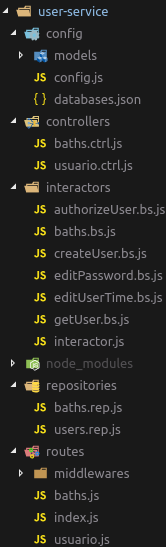
\includegraphics[width=0.22\linewidth]{figuras/cleanarch.png}
	\caption{Divisão dos arquivos do Sistema de Usuários}
	\label{fig:clean}
\end{figure}



\subsection{Sistema de usuários} \label{sec:usuarios}

O propósito desta aplicação está em ter o controle e informações sobre o consumo de água em residências, para isso, é necessário ter um meio para conseguir as informações sobre os usuários do sistema. 

O microsserviço de usuários é responsável por cadastrar e editar usuários, cadastrar informações sobre o tempo de banho do usuário e autorizar o usuário a tomar o banho.

As operações são realizadas através dos \textit{endpoints} (Tabela \ref{tab:endpoints}), que é uma forma de comunicação entre os sistemas. O sistema os disponibiliza como endereços para acesso, que podem receber e enviar informações, dependendo do que foi programado.

Este microsserviço salva todos os dados recebidos nas tabelas do PostgreSQL.

%\begin{itemize} \label{item:endpoints}
%	\item /cadastrar: possibilita cadastrar o usuário com as informações do nome, senha e tempo de banho permitido.
%	\item /autorizar: recebe o id do usuário e a senha, compara a senha enviada com a senha cadastrada e retorna se o usuário está ou não autorizado.
%	\item /editar-tempo: possibilita editar o tempo de banho permitido do usuário.
%	\item /editar-senha: possibilita editar a senha do usuário.
%	\item /banho: salva no banco de dados informações do banho, o tempo e o usuário que tomou o banho.
%	\item /banho/:id: retorna informações sobre todos os banhos do usuário.
%\end{itemize}

% Please add the following required packages to your document preamble:
% \usepackage[table,xcdraw]{xcolor}
% If you use beamer only pass "xcolor=table" option, i.e. \documentclass[xcolor=table]{beamer}
\begin{table}[]
	\centering
	\begin{tabular}{|l|l|}
		\hline
		\rowcolor[HTML]{ECF4FF} 
		\multicolumn{1}{|c|}{\cellcolor[HTML]{ECF4FF}\textit{Endpoint}} & \multicolumn{1}{c|}{\cellcolor[HTML]{ECF4FF}Característica}                                                                                                                      \\ \hline
		/cadastrar                                             & \begin{tabular}[c]{@{}l@{}}possibilita cadastrar o usuário com as informações do nome, senha e\\ tempo de banho permitido\end{tabular}                                   \\ \hline
		/autorizar                                    & \begin{tabular}[c]{@{}l@{}}recebe o id do usuário e a senha, compara a senha enviada com a senha\\ cadastrada e retorna se o usuário está ou não autorizado\end{tabular} \\ \hline
		/editar-tempo                                 & possibilita editar o tempo de banho permitido do usuário                                                                                                                 \\ \hline
		/editar-senha                                 & possibilita editar a senha do usuário                                                                                                                                    \\ \hline
		/banho                                        & \begin{tabular}[c]{@{}l@{}}salva no banco de dados informações do banho, o tempo e o usuário que\\ tomou o banho\end{tabular}                                            \\ \hline
		/banho/:id                                             & retorna informações sobre todos os banhos do usuário                                                                                                                     \\ \hline
	\end{tabular}
	\caption{\textit{Endpoints} do sistema de usuários.}
	\label{tab:endpoints}
\end{table}

Os códigos de implementação deste sistema podem ser observados no Apêndice \ref{ap:users}.

\subsection{Sistema de comunicação MQTT} \label{sec:sistemacomunicacao}

Este microsserviço é responsável pelo recebimento e manipulação dos dados recebidos dos sensores e do teclado numérico via MQTT. Também é responsável por comunicar com o sistema de usuários para a autorização do usuário, ligar ou desligar o atuador, além de salvar os dados no InfluxDB.

O sistema de comunicação recebe informações sobre as teclas digitadas e comunica com o sistema de usuários para autorizar ou não o ligamento do atuador, que significa o início do banho.

O sistema se subscreve nos tópicos do \textit{broker} MQTT descritos na Tabela \ref{tab:topics} para receber e enviar as informações.

%\begin{itemize}
%	\item \textit{keys}: é o tópico em que contém a tecla digitada no teclado numérico
%	\item \textit{actuator}: é o tópico para enviar informações do atuador, para liga-lo ou desliga-lo
%	\item \textit{user}: é o tópico para enviar informações do usuário, como o nome e se ele está autorizado ou não.
%	\item \textit{sensor}: é o tópico para enviar informações do sensor de fluxo.
%\end{itemize}

% Please add the following required packages to your document preamble:
% \usepackage[table,xcdraw]{xcolor}
% If you use beamer only pass "xcolor=table" option, i.e. \documentclass[xcolor=table]{beamer}

\begin{table}[]
	\centering
	\begin{tabular}{|l|l|}
		\hline
		\rowcolor[HTML]{ECF4FF} 
		\multicolumn{1}{|c|}{\cellcolor[HTML]{ECF4FF}Tópico} & \multicolumn{1}{c|}{\cellcolor[HTML]{ECF4FF}Função}                        \\ \hline
		\textit{keys}                                        & contém a tecla digitada no teclado numérico                                    \\ \hline
		\textit{actuator}                                    & envia informações do atuador, para liga-lo ou desliga-lo                       \\ \hline
		\textit{user}                                        & envia informações sobre o usuário, como o nome e se ele está autorizado ou não \\ \hline
		\textit{sensor}                                      & envia informações do sensor de fluxo                                           \\ \hline
	\end{tabular}
	\caption{Tópicos do \textit{broker} MQTT.}
	\label{tab:topics}
\end{table}

Os códigos de implementação deste sistema podem ser observados no Apêndice \ref{ap:mqtt}.

\newpage

\subsection{Sistema de simulação de dados} \label{sec:sistemasimulacao}

O sistema de simulação de dados emula todos os dados que podem ser capturados e enviados ao sistema físico, que são:

\begin{itemize}
	\item Dados do fluxo de água: informação recebida pelo sensor YF-S201 (Seção \ref{sec:sensor});
	\item Dados do teclado numérico: informação de qual tecla foi pressionada (Seção \ref{sec:teclado});
	\item Informações para o atuador: informação para ligar/desligar o atuador (Seção \ref{sec:valvula});
\end{itemize}

Este sistema se inscreve nos tópicos do servidor MQTT e envia os dados simulados como se fosse o próprio sistema físico. Ao se iniciar o sistema, ele fica em estado de espera até alguma tecla for pressionada. Ao se pressionar uma tecla, ele a envia para o tópico \textit{keys}. O Sistema de Comunicação, que se inscreve nesse tópico, reconhece a tecla e toma as devidas ações, como requisitar a senha ou ligar/desligar o atuador.

Os dados do fluxo de água são número inteiros que são passados para o tópico \textit{sensor} do servidor MQTT, para simular estes dados envia-se um valor inteiro ao tópico em um intervalo pre-determinado de tempo (50 ms).

A Figura \ref{fig:mockservice} mostra o sistema de simulação funcionando, com o usuário com o id 3 sendo autorizado e o sinal de ligar/desligar o atuador enviado.

\begin{figure}[htbp]
	\centering
	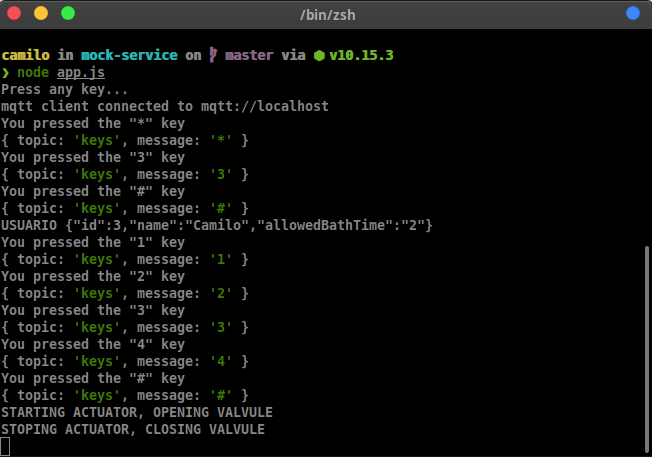
\includegraphics[width=0.6\linewidth]{figuras/mockservice.png}
	\caption{Exemplo do sistema de simulação}
	\label{fig:mockservice}
\end{figure}

\newpage

\section{Configuração do HomeAssistant}

O HomeAssistant pode ser instalado a partir de diversos métodos\footnote{\url{https://www.home-assistant.io/docs/installation}}, neste sistema, a instalação foi feita utilizando o Hassbian, que é um sistema operacional linux para o Raspberry Pi com o HomeAssistant pré-instalado.

Para configurar o HomeAssistant no Raspberry Pi é necessário realizar o download da imagem do Hassbian. Com o download concluído, deve-se copiar a imagem para o cartão SD a ser inserido no Raspberry Pi. Para isto, utilizamos o \textit{balenaEtcher}.

Com a imagem devidamente escrita no cartão SD, basta inseri-lo no Raspberry Pi, configurar a rede como descrito na Seção \ref{sec:confrasp}, e, ao iniciar o sistema, o HomeAssistant será carregado automaticamente.

O HomeAssistant utiliza a porta 8123 e, para conseguir visualizar sua interface, o IP do servidor deve ser acessado por esta porta. No caso deste sistema, o IP do Raspberry Pi foi colocado como estático \textit{192.168.2.60}. Então, para acessar a interface deve-se estar conectado na mesma rede do Raspberry Pi e acessar o link \textit{http://192.168.2.60:8123}, como podemos ver na Figura \ref{fig:homeassistanthome}.

\begin{figure}[htbp]
	\centering
	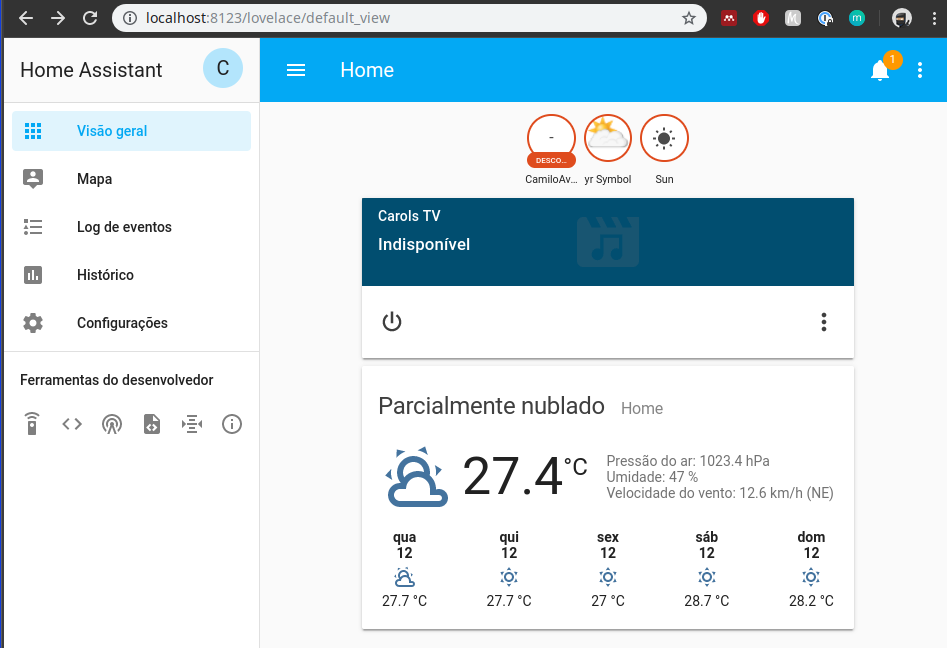
\includegraphics[width=1\linewidth]{figuras/homeassistanthome.png}
	\caption{Página inicial do HomeAssistant acessado por um cliente conectado na mesma rede local do servidor Hassbian.}
	\label{fig:homeassistanthome}
\end{figure}

\subsection{Sensores}

A interface do HomeAssistant permite diversas configurações e inclusão de diferentes sensores, como mostra a Figura \ref{fig:homeassistant-dash}. No sistema desenvolvido neste trabalho, foi utilizado o sensor binário, que mostra o estado do chuveiro como ligado ou desligado. Cada usuário terá um sensor próprio, e seu estado será mostrado na interface.


\section{Configuração do Grafana}

A instalação do Grafana foi realizada através do download\footnote{\url{https://grafana.com/get}} e extração do pacote para o sistema operacional Debian.

Com o pacote devidamente instalado no sistema, o Grafana utiliza a porta 3003 como interface. Para acessá-la, deve-se conectar à porta 3003 do Raspberry Pi, ou seja, acessar o link \textit{http://192.168.2.60:3003}, como na Figura \ref{fig:grafanahome}.

\begin{figure}[htbp]
	\centering
	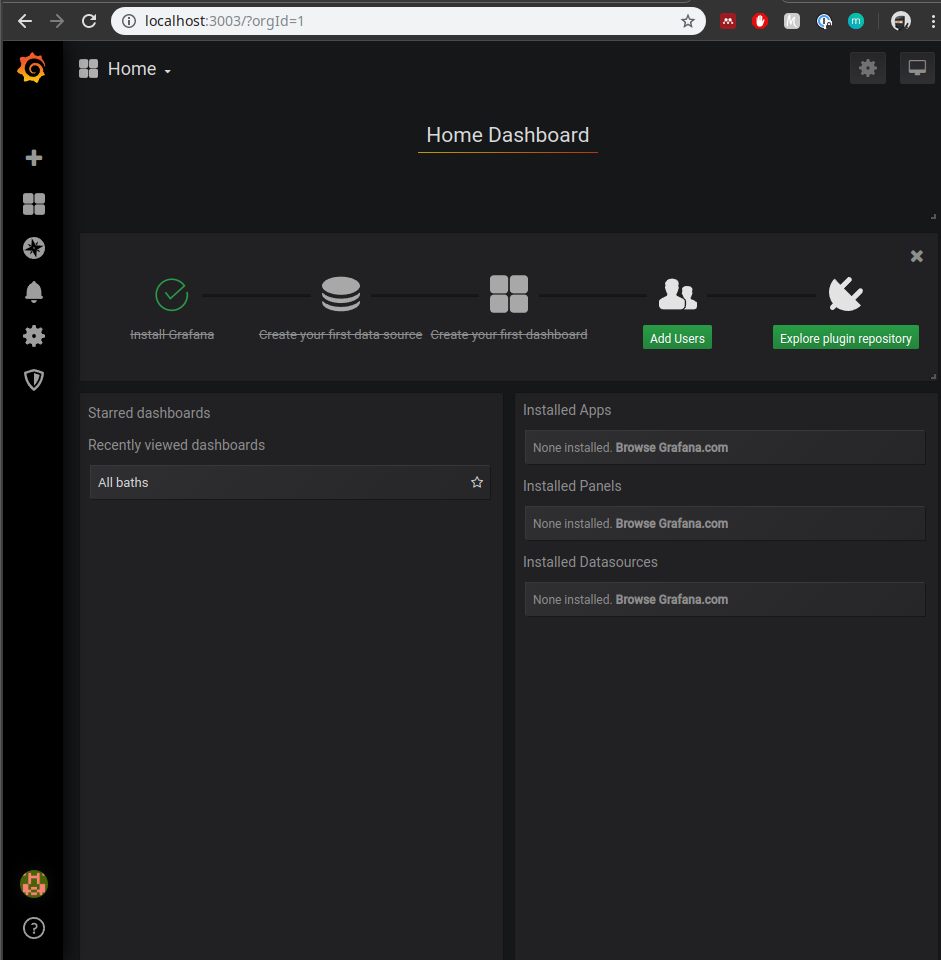
\includegraphics[width=1\linewidth]{figuras/grafanahome.png}
	\caption{Página inicial do Grafana.}
	\label{fig:grafanahome}
\end{figure}

\newpage

Ao acessar a interface do Grafana, é necessário criar um \textit{dashboard}\footnote{\textit{Dashboards} são painéis que mostram métricas e indicadores importantes para alcançar objetivos e metas traçadas de forma visual, facilitando a compreensão das informações geradas.} para a visualização dos dados do InfluxDB. Neste sistema criamos o \textit{dashboard AllBaths}, que se conecta no ip e porta do InfluxDB e realiza as consultas no banco \textit{water\_flow\_data} criado para guardar os dados temporais do fluxo de água.

A configuração do gráfico no Grafana pode ser observada na Figura \ref{fig:grafanaconf}.

\begin{figure}[htbp]
	\centering
	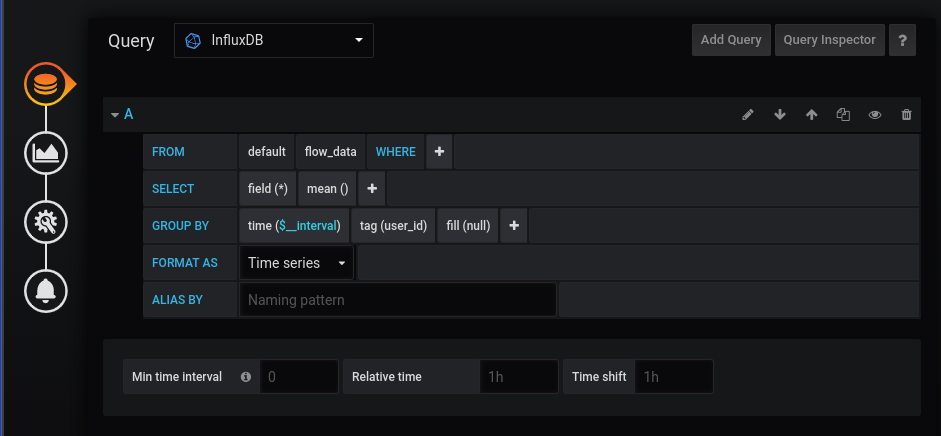
\includegraphics[width=1\linewidth]{figuras/grafanaconf.png}
	\caption{Configuração do gráfico no Grafana.}
	\label{fig:grafanaconf}
\end{figure}

Após a configuração do \textit{dashboard}, um atalho será criado na página inicial do Grafana, e para visualizar os dados, basta clicar neste atalho e será aberto um gráfico com os fluxos medidos no sensor.

%\section{Configuração do Docker}
%
%Toda a configuração do Docker é realizada a partir do arquivo \textit{Dockerfile}, que deve ser criado no diretório do projeto em que se deseja configurar.
%
%No \textit{Dockerfile} alguns parâmetros devem ser passados para conseguir o resultado esperado, um deles é definir qual imagem do Docker será usada como base, no caso dos projetos desenvolvidos, todos utilizam o Node como imagem base, esta imagem é definida com o comando \textit{FROM node}.
%
%Outro parâmetro que precisa ser configurado é o \textit{WORKDIR}, que define o diretório que será usado como base dentro da imagem do Docker, no caso, dentro da imagem do Node.
%
%Um comando importante é o \textit{COPY}, que serve para copiar os arquivos do diretório raiz do Docker, para o \textit{WORKDIR} dentro da imagem do Node.
%
%Após copiar os arquivos, é necessário executar os comandos para instalar os pacotes dos projetos, com o comando \textit{RUN npm install}.
%
%Finalmente, deve-se definir um comando de entrada, que irá executar o projeto dentro da imagem no Docker, que é o comando \textit{CMD npm start}. Caso o projeto utilize alguma porta para configuração, deve-se também expor a porta para garantir o funcionamento com o comando \textit {EXPOSE numeroDaPorta}.
%
%O exemplo do \textit{Dockerfile} do Sistema de Usuários pode ser verificado na Figura \ref{fig:dockerfile}.
%
%\begin{figure}[htbp]
%	\centering
%	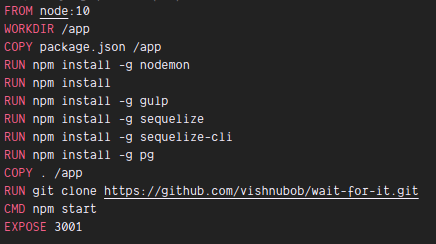
\includegraphics[width=0.7\linewidth]{figuras/dockerfile.png}
%	\caption{Exemplo de \textit{Dockerfile} do Sistema de Usuários}
%	\label{fig:dockerfile}
%\end{figure}
%
%\subsection{Docker-compose}
%
%O \textit{Dockerfile} permite a execução única do projeto em que ele está presente, para iniciar os projetos utilizando apenas o \textit{Dockerfile} é necessário iniciar um por um.
%
%Para contornar este problema, o \textit{docker-compose} permite a execução de todos os projetos com apenas um comando, desde que um arquivo \textit{docker-compose.yml} esteja devidamente configurado. Este arquivo permite também a instalação e configuração automática de todos os programas utilizados neste trabalho, como o PostgreSQL, o InfluxDB, o Grafana e o Mosquitto.
%
%A configuração do \textit{docker-compose.yml} é simples como a do \textit{Dockerfile}, nele, deve-se especificar a versão que deseja utilizar, neste projeto foi utilizada a 3.5, com o comando \textit{version}:"3.5".
%
%Após a definição da versão, deve-se especificar os \textit{services}, que são as imagens que devem iniciar com o Docker. Neste projeto foram utilizados os \textit{builds} dos projetos já implementados com os devidos \textit{Dockerfiles} configurados. 
%
%Além dos projetos já implementados, foram especificados também os programas que foram utilizados no sistema, com o comando \textit{image:}postgres, \textit{image:}homeassistant, \textit{image:}eclipse-mosquitto, \textit{image:}grafana, \textit{image:}influxdb.
%
%O código implementado do \textit{docker-compose.yml} do projeto pode ser verificado no Apêndice C.




% ----------------------------------------------------------
% PARTE
% ----------------------------------------------------------
%\part{Resultados}
% ----------------------------------------------------------
% ---
% primeiro capitulo de Resultados
\chapter{Experimentos e Resultados}

Neste Capítulo encontram-se os experimentos realizados com os sistemas devidamente implementados e configurados. Discutiremos os resultados obtidos, testando os sistemas com todas as suas funcionalidades.

\section{Manipulação de usuários}

O microsserviço de usuários utiliza a porta 3001. Para utiliza-lo e testa-lo, devemos utilizar esta porta juntamente com os \textit{endpoints} disponíveis (Seção \ref{sec:usuarios}). Aqui realizaremos as consultas em todos estes \textit{endpoints} e discutiremos os resultados obtidos.

Para criar um usuário devemos consumir\footnote{O termo "consumir um \textit{endpoint}"\  significa enviar informações para o \textit{endpoint}, esperando algum retorno, de sucesso ou falha.} o \textit{endpoint} http://localhost:3001/usuario/cadastrar passando os parâmetros via \textit{POST} no formato \textit{JSON}\footnote{Javascript Object Notation (JSON), é um formato compacto de troca de dados simples e rápida entre sistema}, como na Figura \ref{fig:cadastro}.

A resposta deste \textit{endpoint} pode ser conferida na Figura \ref{fig:cadastro} e, para garantir que o usuário foi incluído no banco de dados, podemos observar a Figura \ref{fig:cadastro}.

\begin{figure}[htbp]
	\centering
	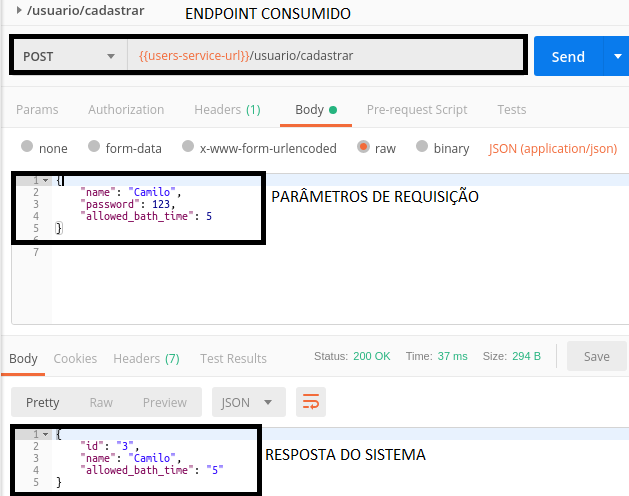
\includegraphics[width=0.7\linewidth]{figuras/postman/cadastro.png}
	\caption{Cadastro de usuários}
	\label{fig:cadastro}
\end{figure}

\clearpage

O \textit{endpoint} http://localhost:3001/usuario/editar-tempo deve ser consumido para editar o tempo máximo de banho de um usuário (Figura \ref{fig:tempo}). Para editar a senha do usuário, deve-se consumir o \textit{endpoint} http://localhost:3001/usuario/editar-senha (Figura \ref{fig:senha}).

\begin{figure}[htbp]
	\centering
	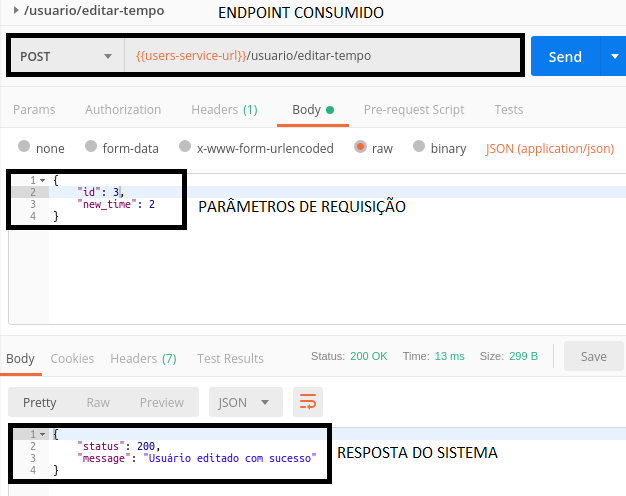
\includegraphics[width=0.7\linewidth]{figuras/postman/time.png}
	\caption{Edição de tempo permitido do usuário}
	\label{fig:tempo}
\end{figure}

\begin{figure}[htbp]
	\centering
	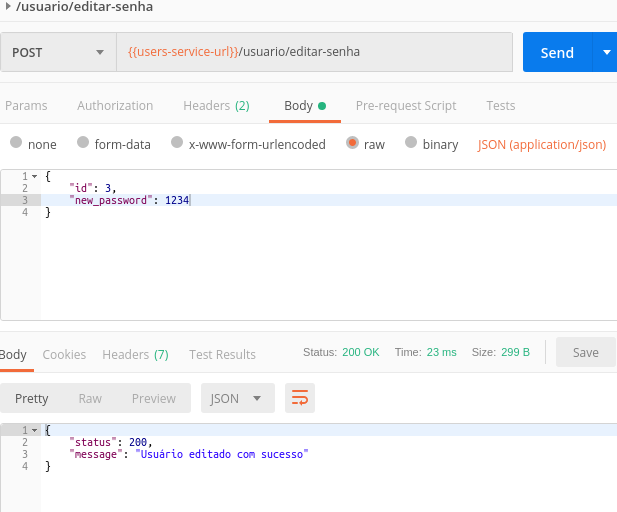
\includegraphics[width=0.7\linewidth]{figuras/postman/password.png}
	\caption{Edição de senha do usuário}
	\label{fig:senha}
\end{figure}

Conseguimos cadastrar um banho ao consumir o \textit{endpoint} http://localhost:3001/banho via \textit{POST} com os parâmetros e resposta mostrados na Figura \ref{fig:banho}.

\begin{figure}[htbp]
	\centering
	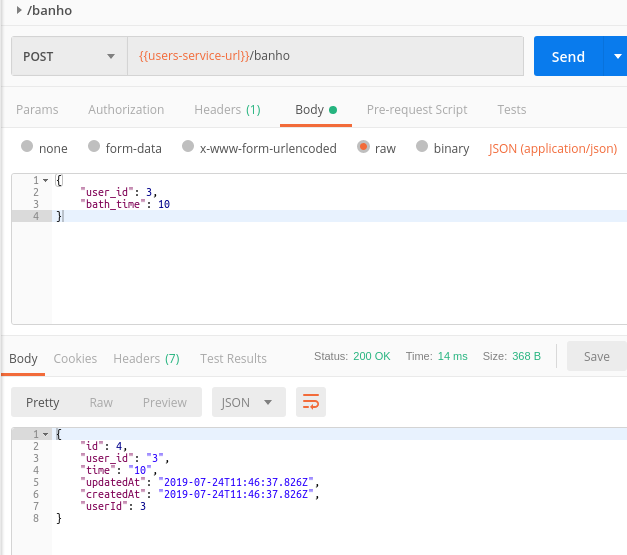
\includegraphics[width=0.7\linewidth]{figuras/postman/bathsinclude.png}
	\caption{Adicionando banhos ao usuário}
	\label{fig:banho}
\end{figure}

Para recuperar as informações de um usuário, basta consumir o \textit{endpoint} \break http://localhost:3001/usuario/idDoUsuario, com o método \textit{GET}, obtendo o resultado da Figura \ref{fig:usuario}.

\begin{figure}[htbp]
	\centering
	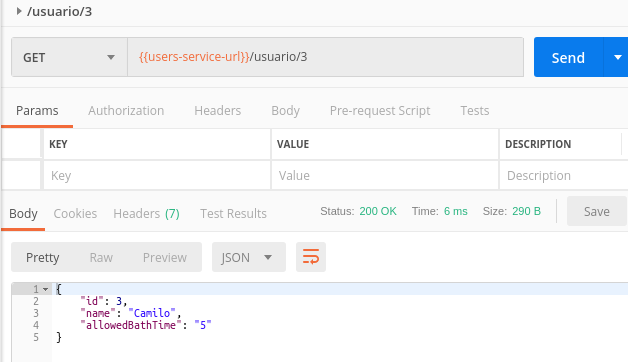
\includegraphics[width=0.7\linewidth]{figuras/postman/getuser.png}
	\caption{Recuperar dados do usuário}
	\label{fig:usuario}
\end{figure}

Conseguimos as informações de todos os banhos dos usuários consumindo o \textit{endpoint} http://localhost:3001/banho/idDoUsuario, via \textit{GET}, e conseguiremos o resultado exibido na Figura \ref{fig:banhos}.

\begin{figure}[htbp]
	\centering
	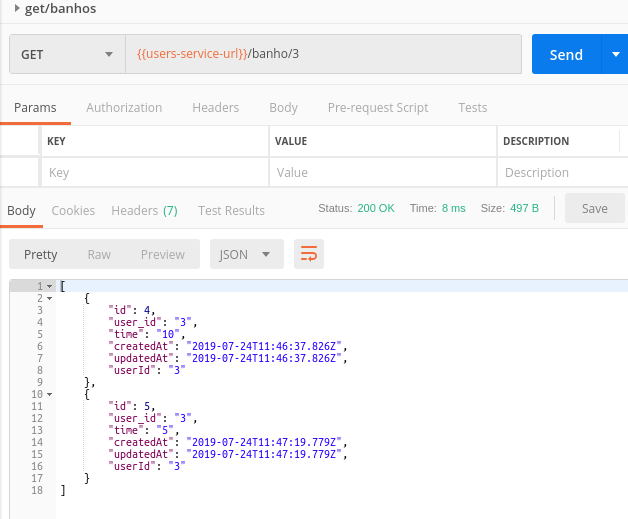
\includegraphics[width=0.7\linewidth]{figuras/postman/getbanhos.png}
	\caption{Recuperar dados de banhos do usuário}
	\label{fig:banhos}
\end{figure}

Finalmente, podemos autenticar os usuários enviando via \textit{POST} os parâmetros para o \textit{endpoint} http://localhost:3001/usuario/autorizar, obtendo como resposta a Figura \ref{fig:allowedtrue}, para usuário autenticado, e Figura \ref{fig:allowedfalse}, para usuário não autenticado, caso a senha esteja errada.

\begin{figure}[htbp]
	\centering
	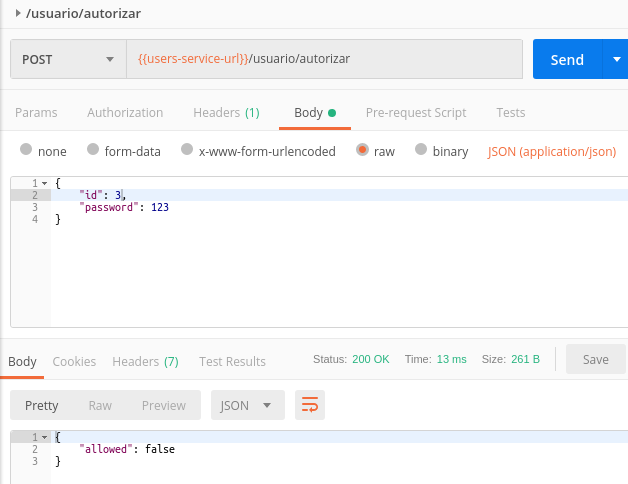
\includegraphics[width=0.7\linewidth]{figuras/postman/allowedfalse.png}
	\caption{Exemplo de usuário não autorizado}
	\label{fig:allowedfalse}
\end{figure}

\begin{figure}[htbp]
	\centering
	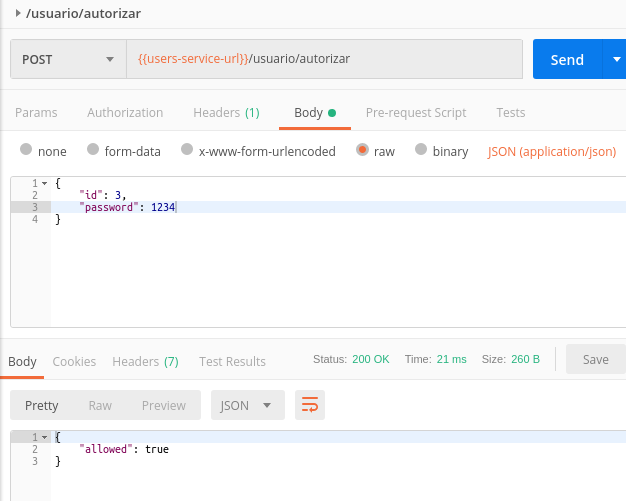
\includegraphics[width=0.7\linewidth]{figuras/postman/allowedtrue.png}
	\caption{Exemplo de usuário autorizado}
	\label{fig:allowedtrue}
\end{figure}

\section{Visualização via Grafana}

Ao autenticar um usuário, o atuador é ativado e o sensor YF-S201 inicia a medição do fluxo, que é automaticamente enviado para o InfluxDB, podendo ser visualizado via Grafana. Os gráficos do grafana podem ser acessados via http://localhost:3003, como na Figura \ref{fig:grafanahome}.

Pode ser observado na Figura \ref{fig:grafana-graph} um gráfico do fluxo medido pelo sensor no horário de 09h30m até 09h35m, por dois usuários diferentes.

\begin{figure}[htbp]
	\centering
	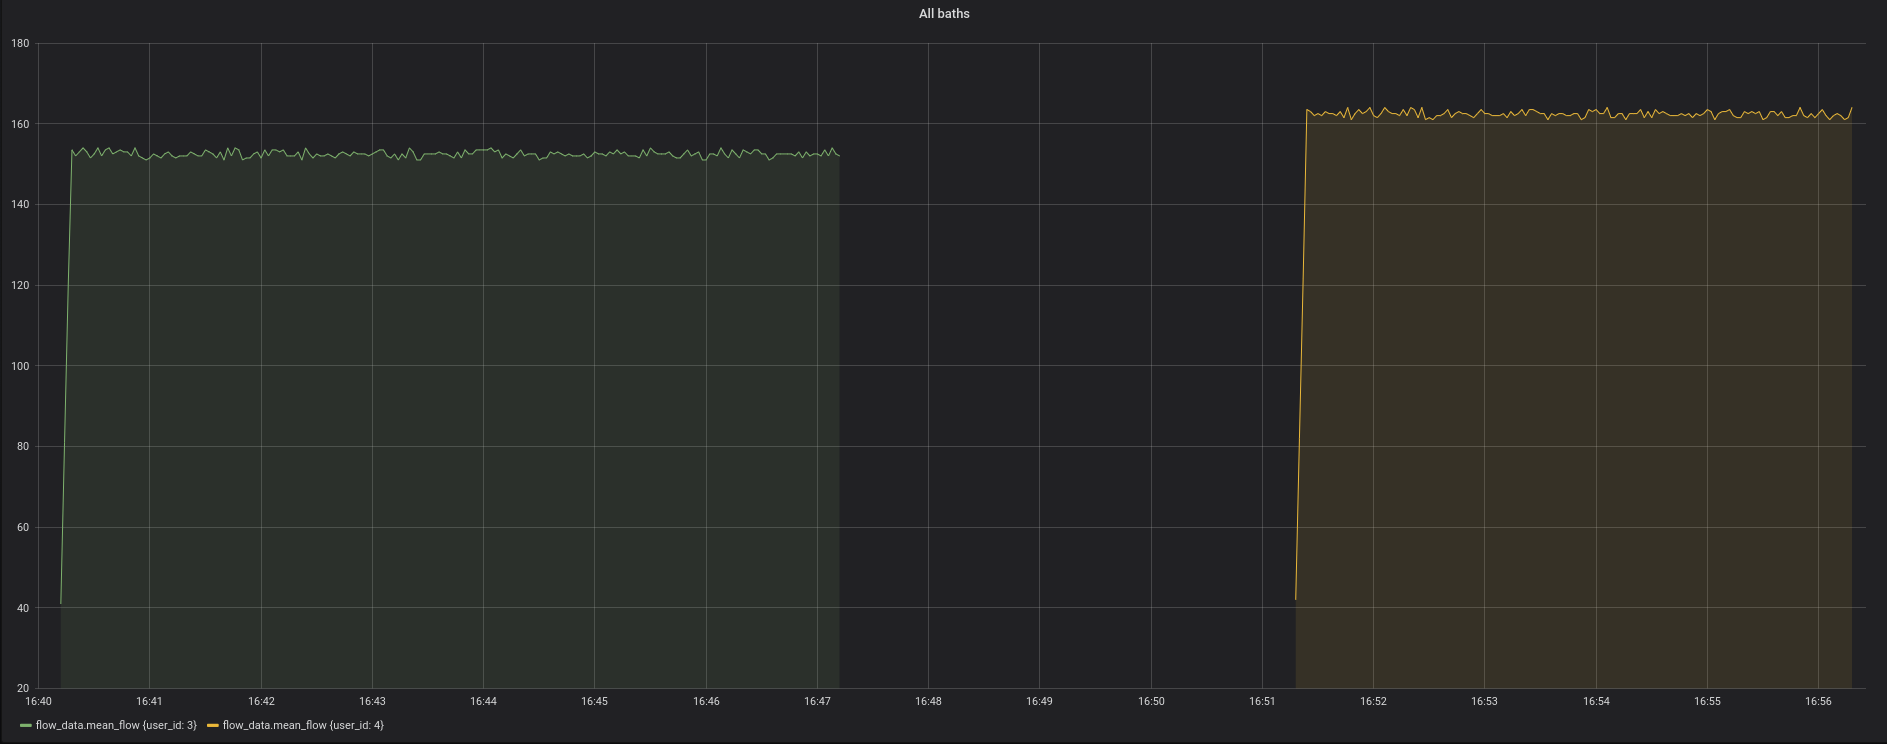
\includegraphics[width=1\linewidth]{figuras/grafanagraph.png}
	\caption{Exemplo do gráfico no Grafana para usuários diferentes}
	\label{fig:grafana-graph}
\end{figure}

\section{Estado do atuador via HomeAssistant}

O HomeAssistant é acessado via http://localhost:8123. Ao acessar o link, observamos os estado dos sensores dos usuários cadastrado na Figura \ref{fig:homeassistant-off}, que encontram-se em estado desligado. Ao digitar corretamente a senha, o estado do sensor muda para ligado, como observado na Figura \ref{fig:homeassistant-on}.

\begin{figure}[htbp]
	\centering
	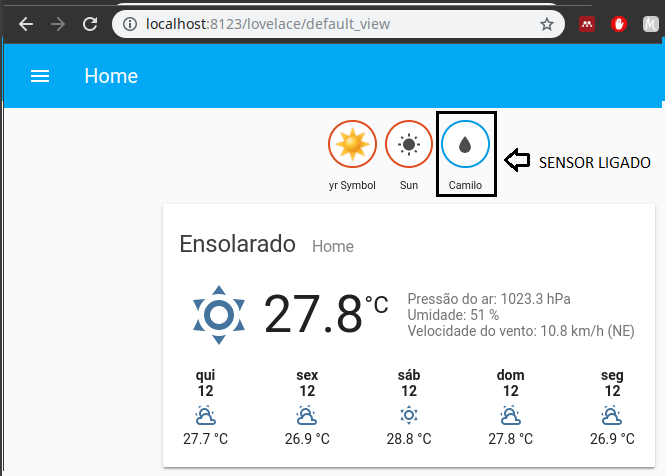
\includegraphics[width=0.6\linewidth]{figuras/homeassistanton.png}
	\caption{Exemplo do sensor no HomeAssistant quando ligado}
	\label{fig:homeassistant-on}
\end{figure}

\begin{figure}[htbp]
	\centering
	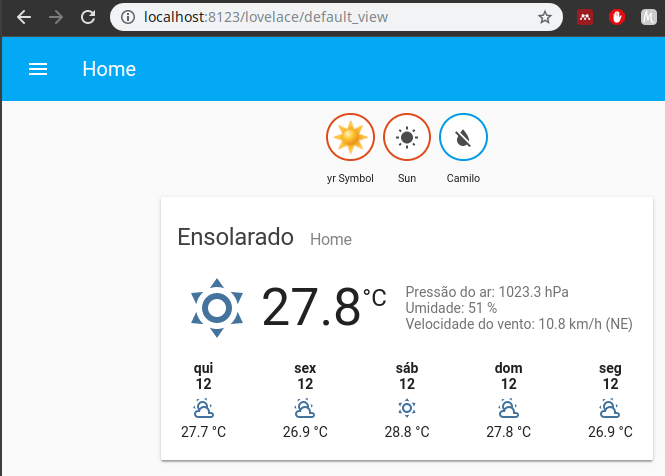
\includegraphics[width=0.6\linewidth]{figuras/homeassistantoff.png}
	\caption{Exemplo do sensor no HomeAssistant quando desligado}
	\label{fig:homeassistant-off}
\end{figure}

Ao cadastrar um usuário, o seu sensor é inserido no HomeAssistant automaticamente (Figura \ref{fig:homeassistant-new}).

\begin{figure}[htbp]
	\centering
	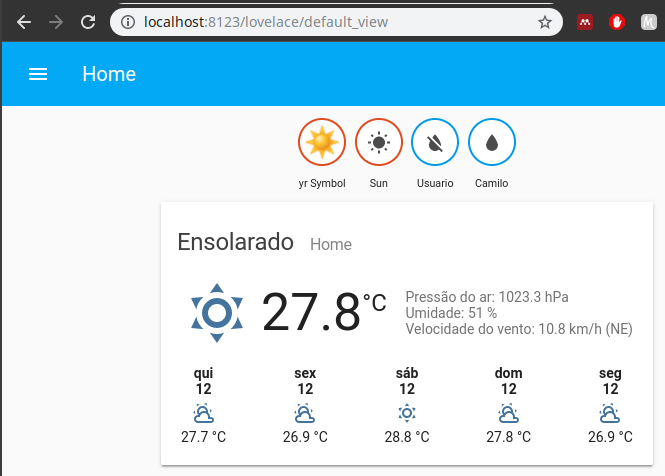
\includegraphics[width=1\linewidth]{figuras/homeassistantnewuser.png}
	\caption{Exemplo de um novo sensor quando um novo usuário é cadastrado}
	\label{fig:homeassistant-new}
\end{figure}



% ----------------------------------------------------------
% Finaliza a parte no bookmark do PDF
% para que se inicie o bookmark na raiz
% e adiciona espaço de parte no Sumário
% ----------------------------------------------------------
%\phantompart
% ---
% Insere arquivo de Considerações Finais ou Conclusões
% ---
\chapter{Considerações Finais}

Este trabalho propõe um sistema capaz de monitorar remotamente a utilização da água em uma residência. Os sistemas de monitoramento propostos foram implementados. Como mostrado, a implementação é capaz de cadastrar, editar e autorizar usuários. Monitorar o fluxo de água e o tempo de banhos com gráficos e estados de sensores em tempo real remotamente, comportando-se como deveria.

O sistema físico não foi criado, devido à necessidade de proteção extra, como caixas resistentes à água e vapores para garantir o seu funcionamento e durabilidade.

Ao final do desenvolvimento do projeto e dos resultados apresentado, pode-se concluir que o sistema é eficaz no monitoramento remoto auxiliando o usuário na gestão da utilização de água em chuveiros. Podendo ser um grande aliado na redução do consumo de água em toda a residência, se implementado em outros setores, como torneiras ou tanques.

Para trabalhos futuros, pode-se realizar a implementação física em chuveiros com sensores e proteção mais robustos que sejam resistentes ao vapor de água presente ao se tomar banho. 

Seria interessante a implementação de mais sistemas de monitoramento utilizando outros sensores realizando a integração com HomeAssistant implementando apenas pequenas modificações e configurações extras. O sistema foi arquitetado e construído com o intuito de facilitar esta inclusão de sensores e reutilização.
% ----------------------------------------------------------
% ELEMENTOS PÓS-TEXTUAIS
% ----------------------------------------------------------
\postextual
% ----------------------------------------------------------
% ----------------------------------------------------------
% Referências
% ----------------------------------------------------------
\bibliography{abntex2-modelo-references}
% ----------------------------------------------------------
% Glossário
% ----------------------------------------------------------
%
% Consulte o manual da classe abntex2 para orientações sobre o glossário.
%
%\glossary

% ----------------------------------------------------------
% Apêndices
% ----------------------------------------------------------
%(Lembre-se: Apendices são de autoria do próprio autor do texto. 
% Anexos são elementos de autorias de outros, que o autor do texto julga interessante apresentar)
% ---
% Inicia os apêndices: 
% ---
\begin{apendicesenv}

% Imprime uma página indicando o início dos apêndices
\partapendices
% ---
% Insere arquivo com os apendices A e B
\chapter{Código sistema de usuários} \label{ap:users}

Neste apêndice encontram-se algumas partes importantes do código do Sistema de Usuários. O código inteiro pode ser baixado no \textit{link}: \url{https://github.com/CamiloAvelar/user-service}

\begin{lstlisting}[caption=Exemplo do código do \textit{interactor} de criação do usuário]
import Interactor from './interactor';
import usersRep from '../repositories/users.rep';
import bcrypt from 'bcrypt';
import config from './../config/config';

class CreateUserBs extends Interactor {
	constructor(){
		super();
	}
	
	async execute({ name, password, allowedBathTime }) {
	
		if (!allowedBathTime) {
			allowedBathTime = 10;
		}
	
		const hash = await bcrypt.hash(password.toString(), config.bcrypt.saltRounds);
	
		const user = await usersRep.createUser({ name, password: hash, allowedBathTime });
		
		if(!user) {
			throw 'Nao foi possivel criar o usuario!';
		}
		
		const response = {
			id: user.user_id,
			name: user.user.name,
			allowed_bath_time: user.allowed_bath_time,
		};
		
		return response;
	}
}

export default CreateUserBs;
\end{lstlisting}

\begin{lstlisting}[caption=Exemplo do código do \textit{interactor} de edição de senha de usuários]
import Interactor from './interactor';
import usersRep from '../repositories/users.rep';
import bcrypt from 'bcrypt';
import config from './../config/config';

class EditPasswordBs extends Interactor {
	constructor(){
		super();
	}
	
	async execute({ id, new_password }) {
	
		const hash = await bcrypt.hash(new_password.toString(), config.bcrypt.saltRounds);
		
		const editedUser = await usersRep.editPassword({ id, password: hash });
		
		const response = editedUser[0] === 1 ? {
			status: 200,
			message: 'Usuario editado com sucesso'
		} : 
		{
			status: 500,
			message: 'Erro ao editar usuario'
		};
		
		return response;
	}
}
\end{lstlisting}

\newpage

\begin{lstlisting}[caption=Exemplo do código do \textit{interactor} de edição de tempo de banho dos usuários]
import Interactor from './interactor';
import usersRep from '../repositories/users.rep';

class EditUserTimeBs extends Interactor {
	constructor() {
		super();
	}
	
	async execute({ id, new_time }) {
	
		const editedUser = await usersRep.editUserTime({ id, new_time });
		
		const response = editedUser[0] === 1 ? {
			status: 200,
			message: 'Usuario editado com sucesso'
		} : 
		{
			status: 500,
			message: 'Erro ao editar usuario'
		};
		
		return response;
	
	}
}
\end{lstlisting}

\newpage

\begin{lstlisting}[caption=Exemplo do código do \textit{interactor} de autorização de usuários]
import Interactor from './interactor';
import usersRep from '../repositories/users.rep';
import bcrypt from 'bcrypt';

class AuthorizeUserBs extends Interactor {
	constructor(){
		super();
	}
	
	async execute({ id, pass }) {
		const user = await usersRep.getUser({ id });
		
		if(!user) {
			throw {error: 'Usuario nao encontrado'};
		}
		
		const match = await bcrypt.compare(pass.toString(), user.password);
		
		return {
			allowed: match
		};
	}
}
\end{lstlisting}

\newpage

\begin{lstlisting}[caption=Exemplo do código do \textit{interactor} de cadastro de banhos]
import Interactor from './interactor';
import bathsRep from '../repositories/baths.rep';

class BathsBs extends Interactor {
	constructor(){
		super();
	}
	
	async execute({ user_id, bath_time }) {
	
		const bath = await bathsRep.createBath({
			user_id,
			bath_time
		});
		
		if(!bath) {
			throw 'Nao foi possivel cadastrar o banho';
		}
		
		return bath;
		}
		
		async getBaths ({ user_id }) {
		
		const baths = await bathsRep.getBaths({
			user_id,
		});
		
		return baths;
	}
}

export default BathsBs;
\end{lstlisting}

\newpage

\begin{lstlisting}[caption=Exemplo do código do \textit{interactor} para recuperar informações dos usuários]
import Interactor from './interactor';
import usersRep from '../repositories/users.rep';

class GetUserBs extends Interactor{
	constructor(){
		super();
	}
	
	async execute({ id }) {
	const user = await usersRep.getUser({ id });
	
	if(!user) {
		throw {error: 'Nao foi possivel localizar o usuario!'};
	}
	
	const response = {
		id: user.id,
		name: user.name,
		allowedBathTime: user.user_setting.allowed_bath_time
	};
	
	return response;
	}
}
\end{lstlisting}

%\begin{figure}[htbp]
%	\centering
%	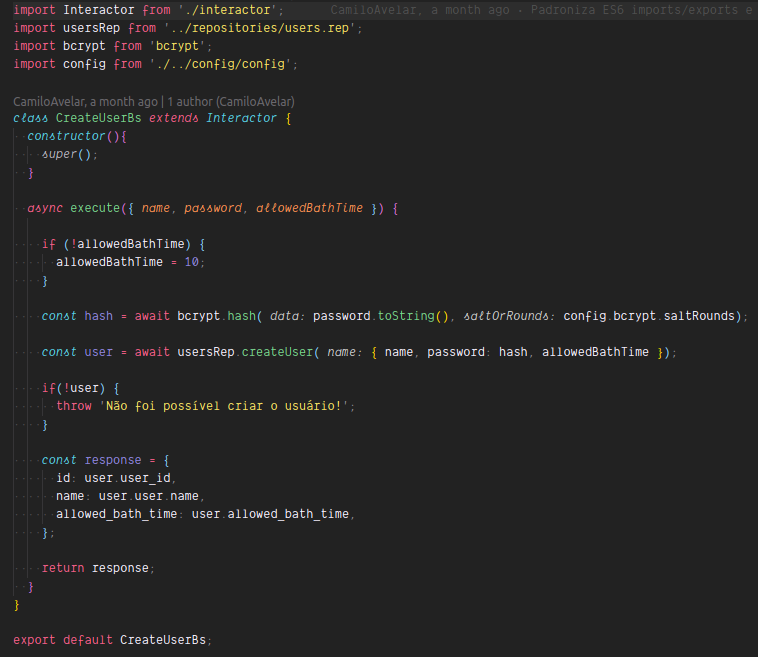
\includegraphics[width=1\linewidth]{figuras/userservice/createuser.png}
%	\caption{Código para criar usuário}
%	\label{fig:createuser}
%\end{figure}
%
%\begin{figure}[htbp]
%	\centering
%	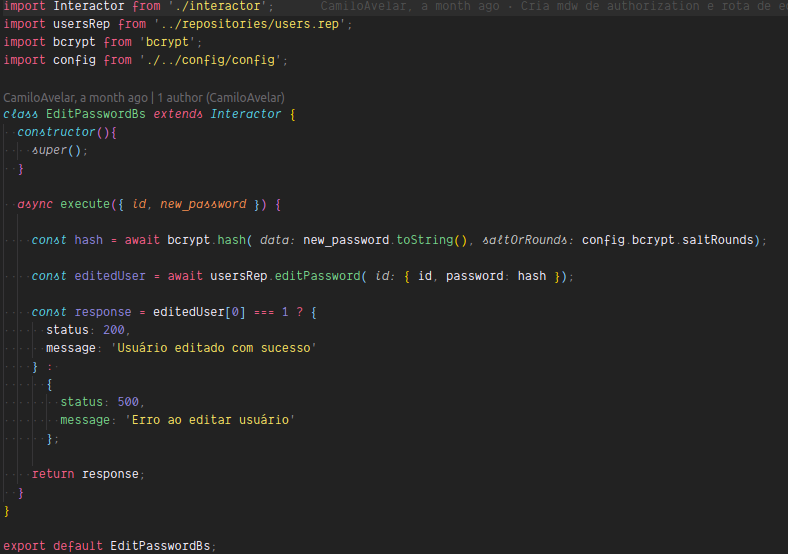
\includegraphics[width=1\linewidth]{figuras/userservice/editpassword.png}
%	\caption{Código para editar senha do usuário}
%	\label{fig:editpass}
%\end{figure}
%
%\begin{figure}[htbp]
%	\centering
%	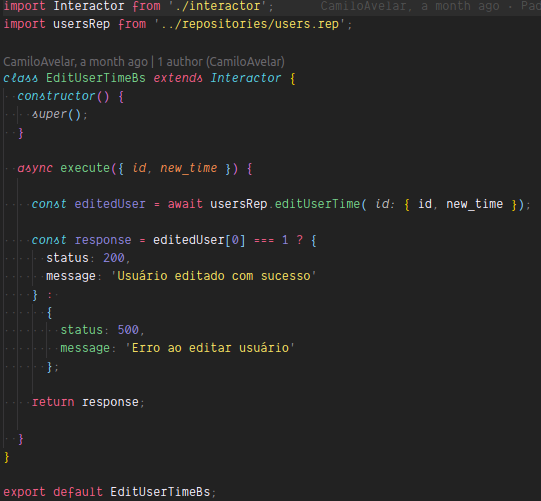
\includegraphics[width=1\linewidth]{figuras/userservice/edittime.png}
%	\caption{Código para editar tempo do usuário}
%	\label{fig:edittime}
%\end{figure}
%
%\begin{figure}[htbp]
%	\centering
%	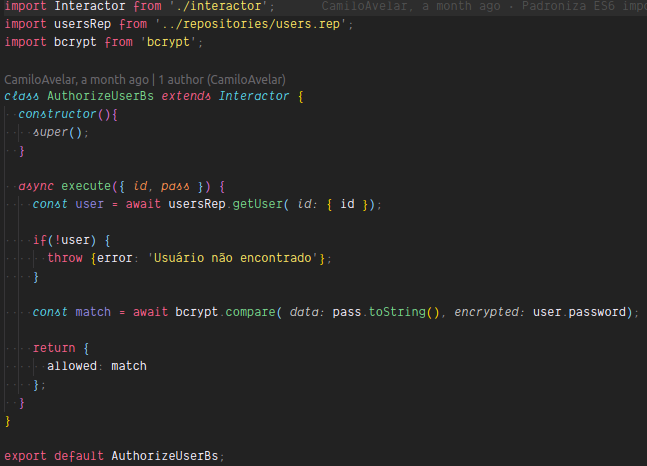
\includegraphics[width=1\linewidth]{figuras/userservice/authorizeuser.png}
%	\caption{Código para autorizar usuário}
%	\label{fig:autorizar}
%\end{figure}
%
%\begin{figure}[htbp]
%	\centering
%	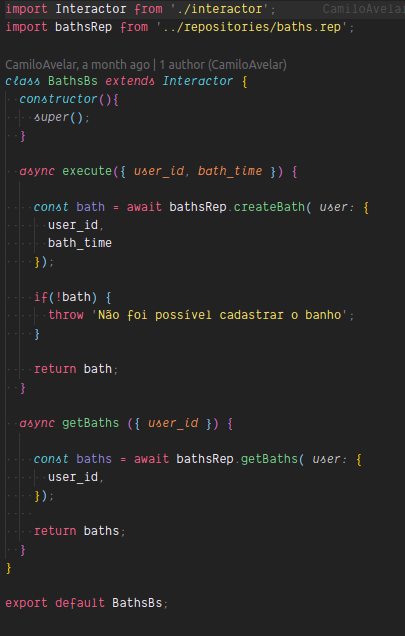
\includegraphics[width=1\linewidth]{figuras/userservice/baths.png}
%	\caption{Código para cadastrar banho do usuário}
%	\label{fig:cadastra-banho}
%\end{figure}
%
%\begin{figure}[htbp]
%	\centering
%	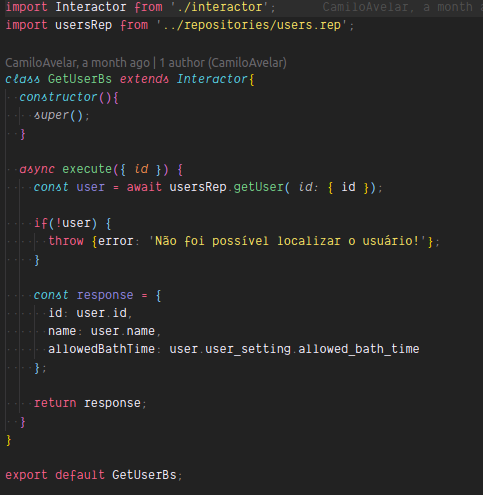
\includegraphics[width=1\linewidth]{figuras/userservice/getuser.png}
%	\caption{Código para recuperar usuários}
%	\label{fig:getuser}
%\end{figure}

\chapter{Código sistema de comunicação MQTT} \label{ap:mqtt}

Neste apêndice encontram-se algumas partes importantes do código do Sistema de comunicação. O código inteiro pode ser baixado no \textit{link}: \url{https://github.com/CamiloAvelar/mqtt-logger-service}

\begin{lstlisting}[caption=Exemplo do código de comunicação MQTT]
const mqtt = require('mqtt');
const EventEmitter = require('events');


class MqttHandler extends EventEmitter {
	constructor() {
		super();
		this.mqttClient = null;
		this.host = 'mqtt://mosquitto';
		this.username = 'mqtt_user'; // mqtt credentials if these are needed to connect
		this.password = '100200300';
	}
	
	
	connect() {
		const self = this;
		this.mqttClient = mqtt.connect(this.host, { username: this.username, password: this.password });
		
		this.mqttClient.on('error', (err) => {
			console.log(err);
			this.mqttClient.end();
		});
		
		this.mqttClient.on('connect', () => {
			console.log(`mqtt client connected to ${this.host}`);
		});
		
		this.mqttClient.on('close', () => {
			console.log(`mqtt client disconnected`);
		});
		
		this.mqttClient.on('message', (topic, message) => {
			const builtMessage = {
				topic,
				message: message.toString()
			};
		
			self.emit('messageReceived', builtMessage);
		})
	}
	
	subscribe(topic) {
		this.mqttClient.subscribe(topic, {qos: 0});
	}
	
	sendMessage(message, topic) {
		this.mqttClient.publish(topic, message);
	}
}

module.exports = MqttHandler;
\end{lstlisting}

\begin{lstlisting}[caption=Exemplo do código responsável por lidar com informações do tempo de banho]
const requestService = require('./requestService');

class timeHandler {
	constructor(mqttClient) {
		this.mqttClient = mqttClient;
		this.allowedTime;
		this.interval;
		this.nowDate;
		this.endDate;
		this.userId;
	}
	
	countTime(allowedTime, id) {
		this.userId = id;
		this.allowedTime = allowedTime;
		this.nowDate = new Date();
		
		this.interval = setInterval(() => {
		this.mqttClient.sendMessage('stop', 'actuator');
		this.clearBathInterval();
		}, this.allowedTime);
	}
	
	async endTime() {
		this.clearBathInterval();
		this.endDate = new Date();
		
		const bathTime = this.endDate - this.nowDate;
		
		console.log('BATHTIME>>>', bathTime);
		await this._requestUserService(bathTime);
	}
	
	clearBathInterval(){
		clearInterval(this.interval);
	}
	
	async _requestUserService(time) {
		const requestOptions = {
			type: 'POST',
			endpoint: 'banho',
			body: {
			user_id: this.userId,
			bath_time: time
			},
		};
		
		return await requestService.userRequest(requestOptions);
	}
}

module.exports = timeHandler;
\end{lstlisting}

\newpage

\begin{lstlisting}[caption=Exemplo do código que lida com a comunicação com o InfluxDB]
const requestService = require('./requestService');

class KeysHandler {
	constructor(mqttClient) {
		this.keyBuffer = '';
		this.working = false;
		this.gettingPassword = false;
		this.userId;
		this.mqttClient = mqttClient;
	}
	
	async handle(message) {
		if(message === '*') {
			this.working = !this.working;
			this.gettingPassword = false;
			return;
		}
	
		if((this.working || this.gettingPassword) && message !== '#') {
			this.keyBuffer += message;
		}
		
		if(message === '#') {
			this.working = false;
			try {
				const response = await this._requestUserService();
				console.log(response);
				this.gettingPassword ? (response.allowed ? this.mqttClient.sendMessage('start', 'actuator') : console.log('NAO AUTORIZADO')) : 
				this.mqttClient.sendMessage(JSON.stringify(response), 'user');
				this.gettingPassword = !this.gettingPassword;
			} catch (err) {
				console.log(err.message)
			} finally {
				this.keyBuffer = '';
			}
		}
	}
	
	async _requestUserService() {
		const requestOptions = this.gettingPassword ? {
			type: 'POST',
			endpoint: `usuario/autorizar`,
			body:{
				id: this.userId,
				password: this.keyBuffer
			},
			}: {
				type: 'GET',
				endpoint: `usuario/${this.keyBuffer}`,
			body: null,
		};
		
		return requestService.userRequest(requestOptions)
		.then((response) => {
			this.userId = this.gettingPassword ? this.userId : response.id;
			return response
		}).catch(err => {throw err});
	}
}

module.exports = KeysHandler;
\end{lstlisting}

%\begin{figure}[htbp]
%	\centering
%	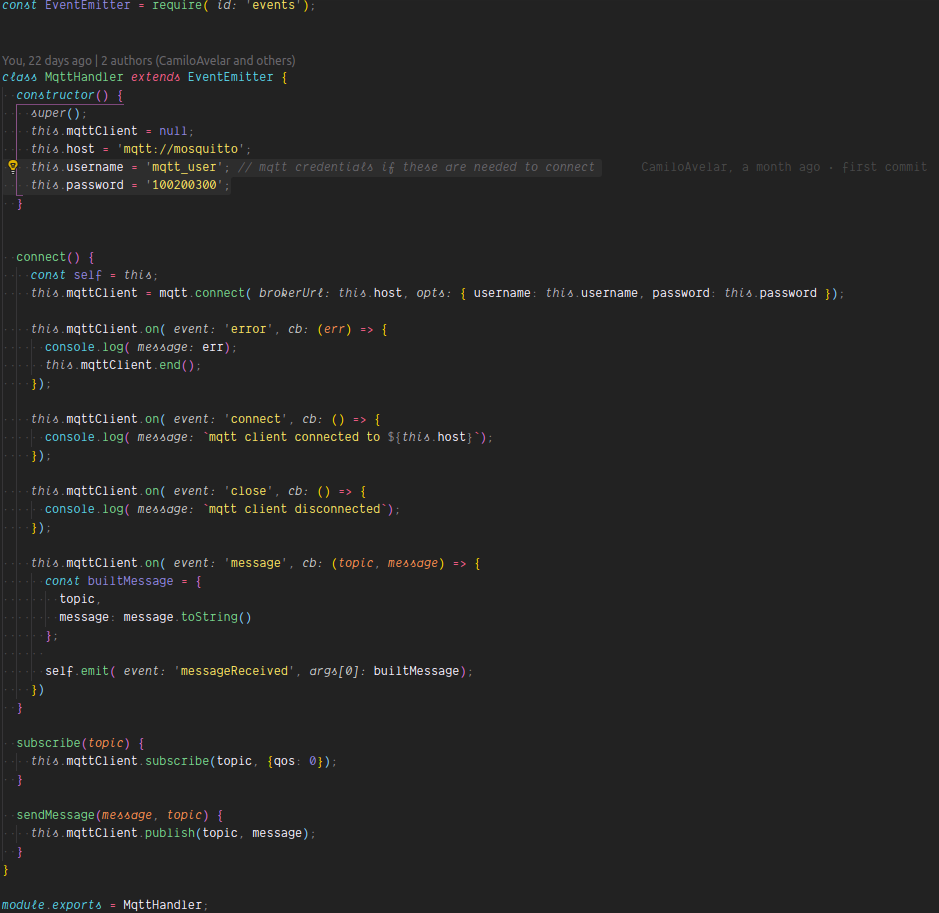
\includegraphics[width=1\linewidth]{figuras/mqttlogger/mqtt.png}
%	\caption{Código para comunicação mqtt}
%	\label{fig:mqtt}
%\end{figure}
%
%\begin{figure}[htbp]
%	\centering
%	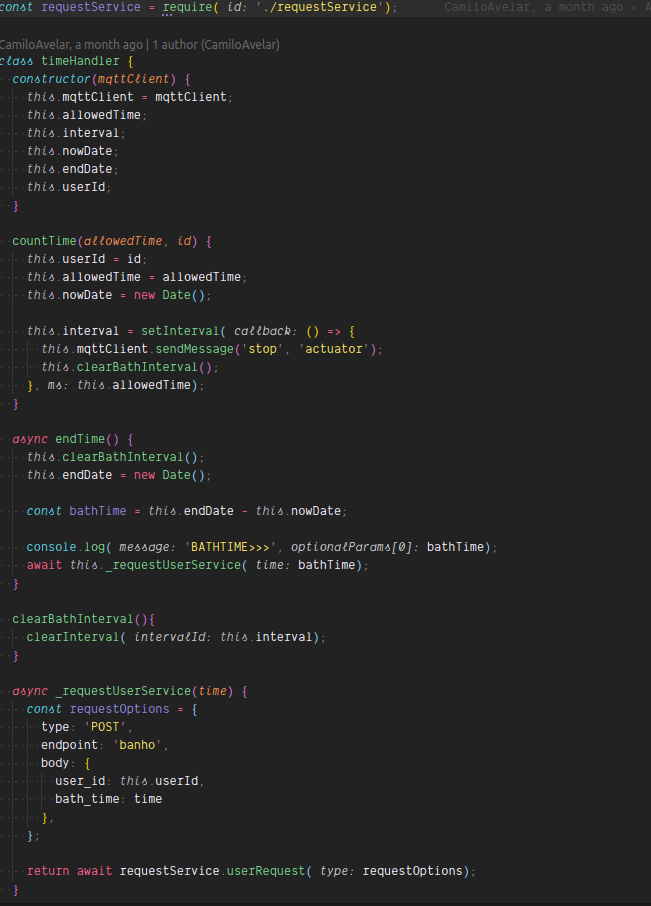
\includegraphics[width=1\linewidth]{figuras/mqttlogger/time.png}
%	\caption{Código que lida com o tempo do banho}
%	\label{fig:time}
%\end{figure}
%
%\begin{figure}[htbp]
%	\centering
%	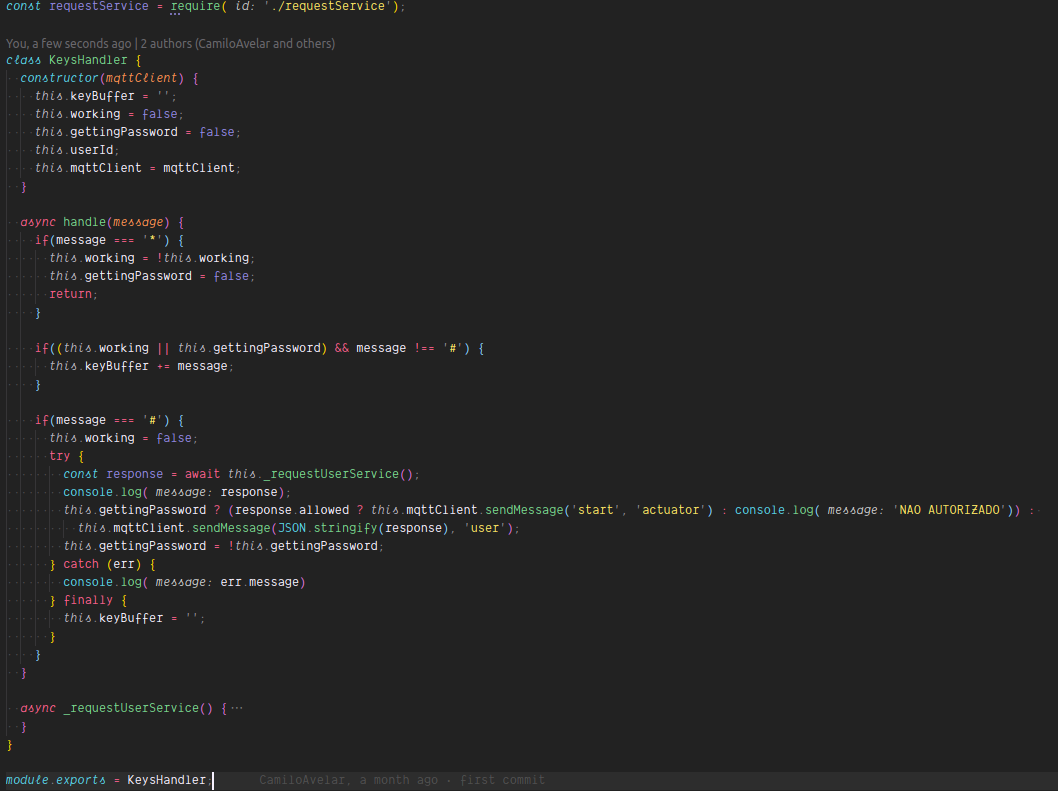
\includegraphics[width=1\linewidth]{figuras/mqttlogger/keystopic.png}
%	\caption{Código que lida com as teclas apertadas no teclado numérico}
%	\label{fig:keys}
%\end{figure}
%
%\begin{figure}[htbp]
%	\centering
%	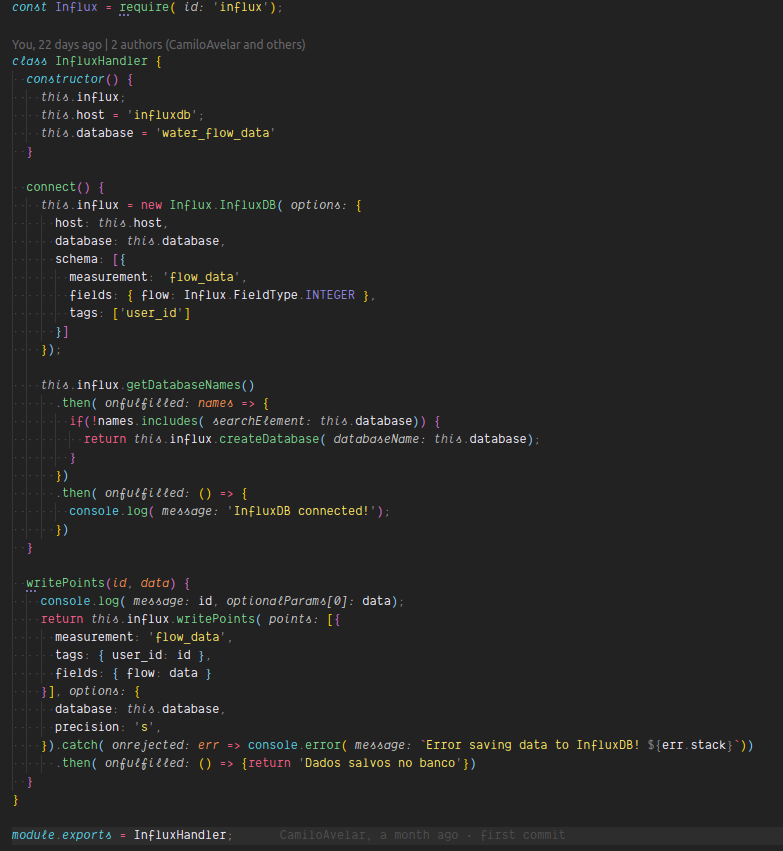
\includegraphics[width=1\linewidth]{figuras/mqttlogger/influx.png}
%	\caption{Código que lida com a comunicação com o InfluxDB}
%	\label{fig:influx}
%\end{figure}

%\chapter{Docker-compose.yml}
%
%\begin{lstlisting}[language=Python]
%version: "3.5"
%
%services:
%	user:
%		build: ./user-service
%		command: gulp
%		depends_on:
%			- postgres
%		volumes:
%			- ./user-service:/app
%		ports:
%			- "3001:3001"
%		networks:
%			- default
%
%	mqtt-logger:
%		build: ./mqtt-logger
%		command: npm start
%		depends_on:
%			- mosquitto
%		volumes:
%			- ./mqtt-logger:/app
%		ports:
%			- "3002:3002"
%
%	postgres:
%		image: postgres
%		restart: always
%		environment:
%		POSTGRES_USER: pi
%		POSTGRES_PASSWORD: 100200300
%		POSTGRES_DB: postgres
%		CONFIGS: "listen_addresses:'*'"
%		volumes:
%			- ./postgres/data:/var/lib/postgresql/data
%		expose:
%			- "5432"
%		ports:
%			- "5432:5432"
%		networks:
%			- default
%
%	migration:
%		image: src_user:latest
%		command: ["./wait-for-it/wait-for-it.sh", "postgres:5432", "--", "npm", "run", "migrate"]
%		links:
%			- postgres
%		depends_on:
%			- postgres
%
%	homeassistant:
%		container_name: homeassistant
%		restart: unless-stopped
%		image: homeassistant/home-assistant
%		volumes:
%			- ./homeassistant:/config
%		depends_on:
%			- mosquitto
%		network_mode: host
%		privileged: true
%		expose:
%			- "8123"
%		ports:
%			- "8123:8123"
%
%	influxdb:
%		image: influxdb:latest
%		container_name: influxdb
%		restart: always
%		ports:
%			- "8083:8083"
%			- "8086:8086"
%			- "8090:8090"
%		volumes:
%			# Data persistency
%			# sudo mkdir -p /srv/docker/influxdb/data
%			- ./influxdb/data:/var/lib/influxdb
%
%	grafana:
%		image: grafana/grafana
%		container_name: grafana
%		restart: always
%		ports:
%			- "3003:3000"
%		links:
%			- influxdb
%		volumes:
%			# Data persistency
%			# sudo mkdir -p /srv/docker/grafana/data; chown 472:472 /srv/docker/grafana/data
%			- ./grafana/data:/var/lib/grafana
%	
%	mosquitto:
%		image: eclipse-mosquitto
%		hostname: mosquitto
%		container_name: mosquitto
%		restart: always
%		user: 1883:1883
%		expose:
%			- "1883"
%			- "9001"
%		ports:
%			- "1883:1883"
%			- "9001:9001"
%		volumes:
%			- ./mosquitto/config:/mosquitto/config
%			# sudo chown 1883:1884 /mosquitto/logs
%			- ./mosquitto/logs:/mosquitto/logs
%		networks:
%			- default
%		networks:
%		default:
%		driver: bridge
%		ipam:
%		config:
%			- subnet: 172.18.1.0/24
%\end{lstlisting}
\end{apendicesenv}
% ---

% ----------------------------------------------------------
% Anexos
% ----------------------------------------------------------
%(Lembre-se: Apendices são de autoria do próprio autor do texto. 
% Anexos são elementos de autorias de outros, que o autor do texto julga interessante apresentar)
% ---
% Inicia os anexos
% ---
\begin{anexosenv}

% Imprime uma página indicando o início dos anexos
\partanexos

% ---
% Insere arquivo com os anexos 1, 2 e 3
\include{capitulos/capitulo-anexos-1-2-3}
% ---
\end{anexosenv}

%---------------------------------------------------------------------
% INDICE REMISSIVO
%---------------------------------------------------------------------
%\phantompart
\printindex
%---------------------------------------------------------------------

\end{document}
